\chapter{Aplikacja demonstracyjna}
\label{chapter:app}

\section{Opis aplikacji wspomagającej warsztat samochodowy}
	
	Nadrzędnym celem aplikacji jest wsparcie dla misji przedsiębiorstwa\footnote{Misja przedsiębiorstwa - zestaw wartości opisujących rolę danego przedsiębiorstwa w jego otoczeniu} prowadzącego warsztat samochody, zajmujący się serwisowaniem samochodów, prowadzącym naprawy, przeglądy i dokonującym okresowych czynności eksploatacyjnych jak na przykład wymiana oleju czy filtrów. Z tego powodu w kolejnych modułach aplikacji została zrealizowana część zarówno serwerowa jak i kliencka dostarczająca funkcjonalności pozwalających na tworzenie, edycję oraz usuwanie obiektów biznesowych, a także przeglądanie informacji o nich. Duży nacisk został położony na zrealizowanie warstwy serwerowej z uwagi na jej krytyczne znaczenie. Jest ona odpowiedzialna za realizację postulatów logiki biznesowej, zarządzanie prawami dostępu, walidację i konwersję danych. Z uwagi na wymienione punkty wiele elementów zostało dopracowanych, a poszczególne autorskie implementacje pewnych problemów zastąpione lepiej przetestowanymi i wydajniejszymi bibliotekami.
		
	\subsection{Funkcjonalność aplikacji}
	W części praktycznej zrealizowane została następująca funkcjonalność:
	\begin{enumerate}
		\item weryfikacja dostępu do konkretnych stron:
		\begin{itemize}
			\item aplikacja rozpoznaje czy użytkownik jest zalogowany, dostosowując ilość dostępnych funkcji,
			w zależności od grupy (grup), w których użytkownik się znajduje,
			\item weryfikacja jest jedno etapowa
		\end{itemize}
		\item tworzenie nowych spotkań,
		\item przeglądanie terminarza spotkań,
		\item tworzenie nowych raportów, zapisywanie ich oraz późniejsze generowanie dla nich wyników,
		\item tworzenie nowych użytkowników:
		\begin{itemize}
			\item nazwa użytkownika oraz hasło,
			\item zestaw ról definiujących poziom uprawnień,
			\item dane kontaktowe
		\end{itemize}
		\item przeglądanie obiektów domenowych jako pojedynczych stron internetowych.
	\end{enumerate}
	
	\subsection{Generyczny moduły} 								Praca nad niewidoczną dla użytkownika końcowego częścią generycznych modułów zaowocowała opracowaniem 3 niezależnych modułów. Działając po stronie serwera upraszczają pracę z takimi elementami, jak strony wyświetlające informacje o obiektach pochodzących z modelu danych, definiowanie nowych tabel i zbioru danych oraz ostatecznie tworzenie, zapisywanie i generowanie raportów biznesowych. 

\subsubsection{Strony obiektów domenowych oraz tabele}
	Komponenty istnieją w dwóch różnych wariantach. Wariant 1 służy do generowania stron dla obiektów biznesowych, zwanych dalej \textbf{info page}, natomiast zadaniem wariantu drugiego jest generowanie zarówno konfiguracji, jak i danych dla tabel. Oba rodzaje zostały zaprojektowane, aby zminimalizować ilość potrzebnych do przesłania danych. Powodem istnienia dwóch różnych klas jest różnica w konstrukcji strony HTML a tabeli. Dodatkowo w przypadku tabeli pewne charakterystyczne elementy, takie jak zmienne opisujące zachowanie kolumn czy też całej tabeli zostały wymuszone przez zastosowanie biblioteki \textbf{Dandelion Datatables} \ref{tech:dandelion}. 
	\begin{listing}[H]
		\inputminted[
			lineos=true,
			firstline=32,
			lastline=46,
			fontfamily=monospace,
			obeytabs=true,
			samepage=true,
			fontsize=\scriptsize
		]{java}{\SpringatomScrPath{/web/component/builders/ComponentBuilder.java}}
		% src file used
		\label{app:component_builder}
		\caption[\textbf{ComponentBuilder - korzeń hierarchii modułu komponentów}]{
			\textbf{ComponentBuilder} - korzeń hierarchii modułu komponentów, który
			wyznacz rolę tego rodzaju obiektów w systemie.					
		}
	\end{listing}
	
	Szczególnie ważne są tutaj następujące metody:
	\begin{itemize}
		\item \textbf{getDefinition()} - wywołanie następuje w momencie kiedy użytkownik otwiera
		stronę, w strukturze DOM, gdzie zapisana jest informacja o obiekcie biznesowym, pobrana z aktualnego adresu
		URL.
		\item \textbf{getData()} - jest to metoda zaprojektowana do wygenerowania
		asynchronicznej odpowiedzi \textbf{Ajax} na żądania pobrania gotowego widoku renderowanego komponentu.
	\end{itemize}

	Z uwagi na dwa oddzielne odnogi \textbf{ComponentBuilder}'ów w strukturze dziedziczenie oraz różnych wymogów, co do konstrukcji końcowego widoku prezentowanego użytkownikowi, istnieją także dwa kontrolery. Jeden z nich został zaprojektowany specjalnie dla \textbf{info page}. Rolą drugiego jest umożliwić generowanie tabel. 

	Poniższe listingi pokazują implementacje metod w warstwie kontrolerów odpowiednio wywołujących funkcje \textbf{getData()} oraz \textbf{getDefinition()}. 
	\begin{listing}[H]
		\inputminted[
			lineos=true,
			firstline=59,
			lastline=79,
			fontfamily=monospace,
			obeytabs=true, 
			samepage=true,
			fontsize=\scriptsize
		]{java}{\SpringatomScrPath{/webmvc/controllers/SVInfoPageController.java}}
		% src file used
		\caption[Obsługa żądania \textbf{ComponentBuilder\#{}getDefinition()}]{
			Obsługa żądania w kontrolerze, które wywołuje metodą \textbf{getDefinition()}
			dla strony domenowej
		}
		\label{app:infopage_ctrl_get_def}
	\end{listing}
	\begin{listing}[H]
		\inputminted[
			lineos=true,
			firstline=89,
			lastline=110,
			fontfamily=monospace,
			obeytabs=true, 
			samepage=true,
			fontsize=\scriptsize
		]{java}{\SpringatomScrPath{/webmvc/controllers/SVTableBuilderController.java}}
		% src file used
		\caption[Obsługa żądania \textbf{ComponentBuilder\#{}getData()}]{
			Obsługa żądania w kontrolerze, które wywołuje metodą \textbf{getData()}
			dla tabeli
		}
		\label{app:table_ctrl_get_data}
	\end{listing}

	Dla tabel istnieje możliwość zdefiniowania atrybutów do zaprezentowania
	użytkownikowi, które bezpośrednio nie istnieją w klasie odpowiadającej danemu obiektowi. Należy wtedy przeciążyć metodę
	\emph{handleDynamicColumn}, której zadaniem jest zwrócenie wartości dla danego, \textbf{dynamicznego} atrybutu.
	Poniższy kod pokazuje przykładową implementację:
	\begin{listing}[H]
		\inputminted[
			lineos=true,
			firstline=75,
			lastline=109,
			fontfamily=monospace,
			obeytabs=true, 
			samepage=true,
			fontsize=\scriptsize
		]{java}{\SpringatomScrPath{/web/rbuilder/table/ReportTableBuilder.java}}
		% src file used
		\caption[Uzyskania wartości dynamicznego atrybutu]{
			Uzyskania wartości dynamicznego atrybutu w momencie tworzenia
			odpowiedzi dla tabeli
		}
		\label{app:handleDynamicColumn}
	\end{listing}
	Zadaniem kodu na listingu \ref{app:handleDynamicColumn} jest zwrócenie akcji dla poszczególnych wierszy, które użytkownik będzie
	mógł wykonać na obiekcie odpowiadającym danemu rekordowi w tabeli. 

\pagebreak
\subsubsection{InfoPage - strony obiektów modelu danych}
	\textbf{InfoPage} jest komponentem prezentującym atrybuty danego obiektu domenowego w postaci strony internetowej. Dzięki wykorzystaniu informacji pobranych z meta modelu obiektów domenowych, utworzenie nowej strony sprowadza się do zaimplementowania rozszerzenia specjalnej klasy \emph{EntityInfoPageComponentBuilder}. Uzyskanie dostępu do danych i wkomponowanie ich do struktury drzewa nie wymaga w tym miejscu dalszej implementacji kodu o ile dany atrybut istnieje w klasie \textbf{Java}. W innym wypadku jest on atrybutem dynamicznym i należy zaimplementować kod, który zwróci jego wartość. Moduł jest wysoce generyczny i zautomatyzowany. Utworzenie strony dla nowego typu w modelu danych, które pojawiły by się w systemie, sprowadza się do utworzenia klasy, gdzie zdefiniowania zostanie struktura strony - panele oraz ich atrybuty. Warto w tym miejscu zaznaczyć, że tak zwany \textbf{panel systemowy} dodawany jest do każdej strony, jeśli powiązany z nią obiekt jest wersjonowany, tj. posiada historię zmian. 
	\begin{figure}[H]
		\centering
		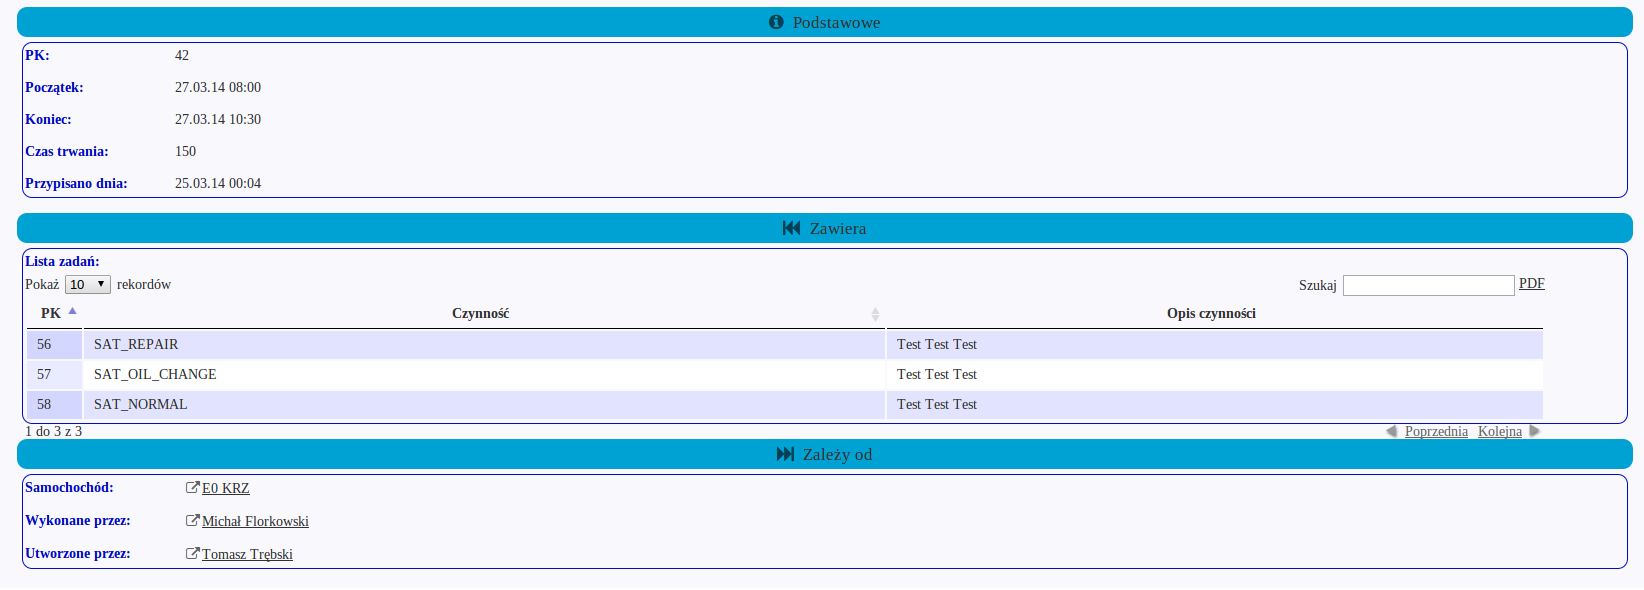
\includegraphics[width=1.0\textwidth]{images/infoPage}
		\caption[Strona domenowa dla spotkania]{
			Strona domenowa dla spotkania	
		}
		\label{app:infoPage}
	\end{figure}
	Na rysunku \ref{app:infoPage} pokazana została strona domenowa obiektu opisującego pojedyncza wizytę w warsztacie samochodowym. Zdefiniowane zostały 3 panele z atrybutami. Panel podstawowy oraz dwa opisujące relacje zachodzące między spotkaniem a innymi obiektami. Spotkanie posiada więc listę zadań oraz zostało przypisane do pewnego samochodu, zgłoszone i wykonane przez konkretnych mechaników. Listing kodu \ref{app:infoPageSrcCode} przedstawia kod Java odpowiedzialny za zbudowania struktury strony.
	\begin{listing}[H]
		\inputminted[
			lineos=true,
			firstline=37,
			lastline=76,
			fontfamily=monospace,
			obeytabs=true,
			samepage=true,
			fontsize=\scriptsize
		]{java}{\SpringatomScrPath{/webmvc/pages/builders/AppointmentInfoPageComponentBuilder.java}}
		\caption[Strona domenowa dla spotkania - kod źródłowy]{Strona domenowa dla spotkania - kod źródłowy}
		\label{app:infoPageSrcCode}
	\end{listing}

\pagebreak
\subsubsection{TableBuilder - definiowanie oraz dane dla tabel}
	Rzadko zdarza się żeby aplikacja nie wymagała korzystania z tabel do prezentowania danych. Są one szczególnie użyteczne zwłaszcza w momencie, kiedy ilość możliwych obiektów do jednorazowego wyświetlenia sięga co najmniej kilkudziesięciu elementów. W części praktycznej za obsługę tabel odpowiada biblioteka \textbf{Dandelion Datatables}. Renderowanie tabel oraz wsparcie dla funkcji takich jak sortowanie, filtrowanie. Niemniej ta biblioteka, podobnie jak wiele innych, nie posiada bezpośredniego wsparcia dla generowania struktur tabel oraz danych po stronie serwera, ze szczególnym naciskiem na definicję tabeli. Moduł \textbf{TableBuilder} rozwiązuje problemy takie jak:
	\begin{itemize}
		\item dynamiczna struktura tabel - to jakie kolumny będą widocznie zależne jest od dowolnych czynników,
		\item wsparcie dla sortowania po stronie serwera,
		\item wsparcie dla filtrowania po stronie serwera,
		\item zwracania danych tekstowych dla kolumn odpowiadających danym nie atomowym\footnote{Obiekt atomowy - pojedynczy, jeden. Obiekt nie atomowym to obiekt zwierający więcej niż jedną informację na raz},
		\item wsparcie dla dynamicznych kolumn, które nie odpowiadają żadnej z cech obiektów wyświetlanych w danej tabeli
	\end{itemize}
		
	\begin{listing}[H]
		\inputminted[
			lineos=true,
			firstline=35,
			lastline=76,
			fontfamily=monospace,
			obeytabs=true,
			samepage=true,
			fontsize=\scriptsize
		]{java}{\SpringatomScrPath{/webmvc/pages/builders/CarsTableBuilder.java}}
		% src file used
		\caption[Klasa definiująca strukturę tabeli wyświetlającej listę samochodów]{
			\emph{CarsTableBuilder} - klasa definiująca strukturę tabeli wyświetlającej listę samochodów	
		}
		\label{app:cars_table_src_code}
	\end{listing}
	
\subsubsection{RBuilder - raporty biznesowe}
	\textbf{RBuilder} jest praktyczną realizacją, będącej na wczesnym etapie rozwoju, koncepcji zaprojektowania generycznego
	silnika raportowania dla aplikacji internetowej. Głównymi założeniami tego komponentu są:
	\begin{itemize}
		\item możliwość generowania raportów przez użytkowników systemu,
		\item możliwość zapisywania raportów do bazy danych, celem późniejszego ich użycia,
		\item możliwość edycji istniejących raportów,
		\item możliwość usuwania istniejących raportów,
		\item wsparcie dla zabezpieczenie akcji możliwych do wykonania na raportach,
		\item eksport raportów do formatów:
		\begin{itemize}	\label{app:rbuilder_representations}
			\item PDF
			\item XLS
			\item HTML
			\item CSV
		\end{itemize}
	\end{itemize}		
	Jest to obecnie najbardziej skomplikowany komponent aplikacji, którego złożoność jeszcze wzrośnie, z uwagi
	na założenie, że raporty mogą być definiowane przez użytkowników. 
	
	Definiowanie raportu przebiega według następujących kroków:
	\begin{enumerate}
		\item Użytkownik wybiera z listy tabele dla których chce wygenerować raport,
		\item Dla zaznaczonych tabel użytkownik wybiera kolumny oraz format, w jakim zostaną wyświetlone,
		\item Użytkownik podaje informacje takie jak:
		\begin{itemize}
			\item nazwa
			\item opis
		\end{itemize}
		\item Sterowanie jest przekazywane do serwisu odpowiedzialnego za:
		\begin{itemize}
			\item zdecydowanie o rodzaju raportu: dla jednej tabeli, dla wielu tabel,
			\item utworzenie obiektu domenowego raportu zawierającego informację takie jak tytuł,
			\item utworzenie, kompilacja i zapisanie zserializowanego obiektu klasy \textbf{DynamicReport} do systemu plików,
			\item zwrócenie sterowania do \textbf{Spring Web Flow}
		\end{itemize}
		\item Generowanie raportu jest dostępne z tabeli zawierającej listę wszystkich raportów
	\end{enumerate}
	
	Report należy w tym miejscu rozumieć jako obiekt domenowy, który służy do późniejszego zapisanie
	wymaganych informacji do bazy danych oraz jako obiekt \textbf{Dynamic Jasper Report}. Celem dla którego
	tworzony jest ten obiekt leży w wykorzystanej bibliotece \textbf{DynamicJasper}. 
	Aby raport mógł być zaprezentowany użytkowniki, musi on zostać w pierwszej kolejności
	skompilowany do pliku \textit{*.jasper}. Załadowanie, a dokładniej odczytanie tego obiektu z zserializowanego
	pliku, zapisanego w systemie plików, jest wymogiem koniecznym i dostatecznym, aby sterowanie procesem
	tworzenie jednej z reprezentacji przekazać do szkieletu aplikacji \textbf{Spring}. Niemniej nie jest to jedyny
	wymóg. W specjalnej mapie, pod jasno określonymi kluczami, musi znaleźć się źródło danych dla raportu spójne z jego budową.
	Powyższe powody generują wiele niedogodności takich jak konieczność przechowywania dodatkowych plików na serwerze oraz
	trudności w uogólnieniu niektórych aspektów projektowania nowego raportu.
	
	Model danych przeznaczony dla \textbf{RBuilder} jest pewnym rozszerzeniem informacji o 
	danych biznesowych (domain object). Zawarte w nim informacje pozwalają na stwierdzenie następujących
	właściwości obiektów domenowych:
	\begin{itemize}
		\item nazwa tabeli,
		\item lokalizowana nazwa tabeli,
		\item atrybuty,
		\item powiązania z innymi modelami.
	\end{itemize}
	
	Późniejsze instancje obiektów zaprezentowanych na diagramie UML są wykorzystywane do przechowywania
	informacji niezbędnych do prawidłowego utworzenia konfiguracji raportu \textbf{ReportConfiguration}.
	
	\begin{figure}[H]
		\centering
		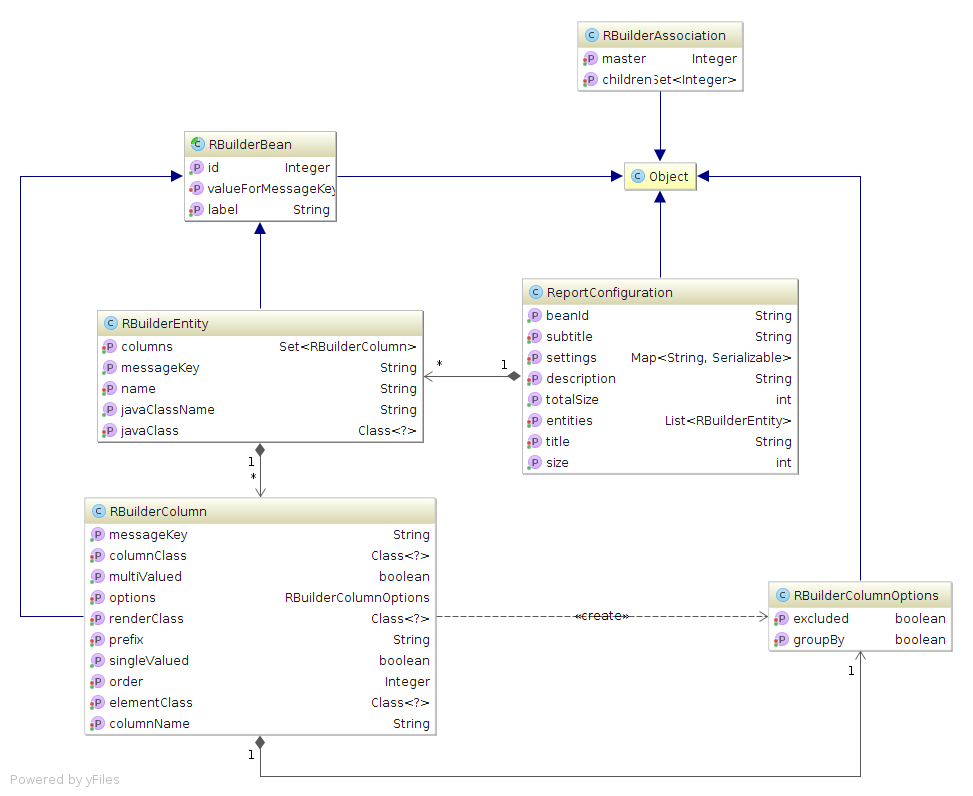
\includegraphics[width=1.0\textwidth]{images/rbuilder_dataModel}
		\caption[Diagram UML modelu danych \textbf{RBuilder}]{
			Diagram UML modelu danych \textbf{RBuilder}
		}
		\label{app:rbuilder_data_Model}
	\end{figure}	
	
	Serwisy \textbf{RBuilder}'a dostarczają metod, dzięki którym możliwe jest przygotowanie gotowego raportu
	w wybranej przez użytkownika reprezentacji i wsparcia dla przewodnika tworzenia nowego raportu. Dostarczone usługi to:
	\begin{itemize}
		\item ustalenie możliwych formatów danego atrybuty, a tym samym kolumny w raporcie,
		\item tworzenie obiektu domenowego w zależności od konfiguracji raportu,
		\item generowanie raportu,
		\item zapis i odczyt informacji o raporcie z bazy danych oraz systemu plików.
	\end{itemize}
	Funkcjonalność tej grupy klas dla komponentu \textbf{RBuilder} można podzielić na następujące bloki:
	\begin{center}
		\begin{longtable}{| p{2.5cm} | p{13cm} |}
			\caption[Bloki funkcjonalne modelu serwisów \textbf{RBuilder}]{
				Bloki funkcjonalne modelu serwisów \textbf{RBuilder}			
			}
			\label{app:rbuilder_services_functionality_table}
			\tabularnewline	
			
			\hline
				\multicolumn{1}{|c|}{\textbf{Grupa}} &
				\multicolumn{1}{|c|}{\textbf{Funkcjonalność}} \tabularnewline
			\hline
			\endfirsthead
			
			\multicolumn{2}{c}
			{{\bfseries \tablename\ \thetable{} -- kontynuacja...}} \tabularnewline
			\hline
				\multicolumn{1}{|c|}{\textbf{Grupa}} &
				\multicolumn{1}{|c|}{\textbf{Funkcjonalność}} \tabularnewline
			\hline
			\endhead
				
			\hline
				\multicolumn{2}{|r|}{{Następna strona...}} \tabularnewline \hline
			\endfoot
			\hline
			\endlastfoot	
			
			\emph{Operation Management} 									& 
			Grupa \textbf{Operation Management} odpowiedzialna jest za tworzenie obiektu \textbf{SReport} w zależności
			od ilości tabel wybranych dla konkretnego raportu. Lista klas:
			\begin{itemize}
				\item RBuilderOperation
				\item RBuilderCreateOperation
				\item SingleEntityRBuilderCreateOperation
				\item MultipleEntitiesRBuilderCreateOperation
			\end{itemize}					
			\hline
			\emph{Data Management}											&
			Klasy z grupy \textbf{Data Management} zostały zaprojektowane do pobierania danych takich jak:
			\begin{itemize}
				\item informacje o typach obiektów domenowych, które można uwzględnić w raportach. Takie klasy adnotowane są 
				przez \emph{\@{}ReportableEntity}, a ich lista udostępniana jest poprzez interfejs \emph{ReportableEntityResolver},
				\item listę kolumn wraz z ich cechami takimi jak nazwa, typ danych rzechowywanych w odpowiadającej jej polu w klasie, odpowiednie typu na które można rzutować dany typ. Informacje tego typu udostępniane są poprzez interfejs \emph{ReportableBeanResolver},
				\item listę powiązań między modelami w uproszczonej formie na potrzeby wybierania tabel podczas projektowania raportu. 
				Na obecną chwile możliwe jest utworzenie jedynie nieprzechodnich powiązań opisanych na bazowym poziomie przez relacje
				klucz główny - obcy. Dane tego typu udostępnione są przez interfejs \emph{ReportableAssociationResolver}. 
			\end{itemize}
			\hline
			\emph{Dynamic Jasper Operation}								&
			\emph{JasperBuilderService} jest jedyną klasą tej grupy, dostarczającą możliwości utworzenia skompilowanego
			raportu typu \textbf{JasperReport}, który potem jest serializowany do systemu plików. Niemniej jej głównym zadaniem
			jest wkomponowanie w obiekty wyżej wymienionego typu takich danych jak:
			\begin{itemize}
				\item tytuł,
				\item podtytuł,
				\item opis,
				\item język,
				\item szerokość odpowiednich sekcji jak nagłówek, stopka itp.,
				\item lista kolumn,
				\item lista kolumn według których dane mają być grupowane.
			\end{itemize}
			\hline
			\emph{View helper}												&
			\emph{ReportBuilderService} jest interfejsem serwisu, którego celem istnienia jest przekazanie sterowania do modułu
			\textbf{Operation Management}, celem utworzenia instancji obiektu domenowego \textbf{SReport} oraz wsparcie
			dla operacji renderowania raportu w konkretnej reprezentacji. Kiedy pierwsza z funkcji jest trywialna w kontekście złożoności, służąc
			jedynie separacji zadań i zmniejszeniu kohezji klas, druga z wymienionych metod jest dużo bardziej złożona.
			Jej celem jest pobranie danych wymaganych przez moduł \textbf{Spring}, używanych później do zrenderowania raportu 
			w wybranej reprezentacji, na przykład PDF. Operacje przez nią wykonywane to:
			\begin{itemize}
				\item pobranie obiektu domenowego z bazy danych dla danego numeru raportu, 
				\item deserializacja skompilowanego pliku \textit{*.jasper} z systemu plików,
				\item utworzenie źródła danych na podstawie informacji takich jak lista kolumn, ich typ, wybranych typ reprezentacji danych w kolumnie
			\end{itemize}
			\hline
		\end{longtable}
	\end{center}
				 
	Na część obsługującą widok komponentu \textbf{RBuilder} składają się:
	\begin{itemize}
		\item tabela z istniejącymi raportami \label{app:rbuilder_table},
		\item przewodnik tworzenia nowego raportu \label{app:rbuilder_wizard},
		\item specjalnie skonfigurowany \textbf{ViewResolver} \footnote{\href{http://docs.spring.io/spring/docs/current/javadoc-api/org/springframework/web/servlet/ViewResolver.html}{ViewResolver} - interfejs, które implementują specjalne klasy zadaniem których jest ładowanie widoków poprzez odwołanie m.in. do plików JSP, logicznych nazw widoków itp.}.
	\end{itemize}

	Tabela (\ref{app:rbuilder_table}) jest obiektem należącym do warstwy widoku, który został utworzony z użyciem komponentu
	tabeli. Zawiera ona dodatkowo akcje, umożliwiające operacje na raportach. 
	% dodać IMG			
	
	Przewodnik (\ref{app:rbuilder_wizard}) został zaprojektowany na podstawie \textbf{Spring Web Flow}. Dzięki 
	temu zbiór formularzy, na których definiuje się poszczególne elementy składowe gotowego obiektu \textbf{ReportConfiguration}
	(stanowiącego bazę do generowania wybranej reprezentacji \ref{app:rbuilder_representations} reportu), jest logicznie
	połączony. Dodatkową korzyścią jest uzyskanie bezproblemowego wsparcia dla przetwarzania danych wejściowych 
	po stronie serwera bez konieczności pisania własnej logiki do zarządzania komunikacją Ajax oraz możliwość przekazywania
	danych między kolejnymi krokami. 
	\begin{figure}[H]
		\centering
		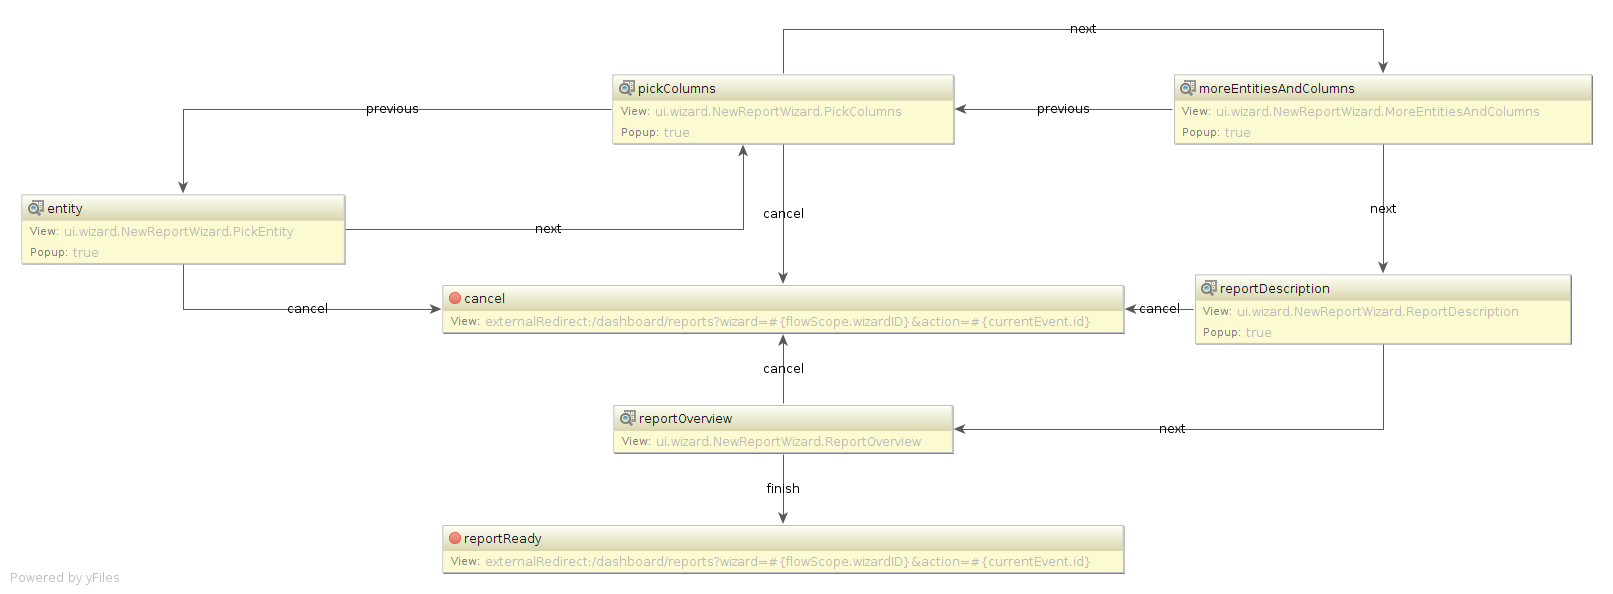
\includegraphics[width=1.0\textwidth]{images/rbuilder_flow}
		\caption[Logiczne połączenie kroków w przewodniku dla \textbf{RBuilder}]{
			Logiczne połączenie kroków w przewodniku dla \textbf{RBuilder}
		}
		\label{app:rbuilder_diagram_of_flow}
	\end{figure}
	Każdy z kroków przewodnika wspiera odpowiednia klasa Java, będąca specjalizowanym rozszerzeniem \href{http://docs.spring.io/spring-webflow/docs/2.4.0.M1/api/org/springframework/webflow/action/FormAction.html}{FormAction}, zarządzającą ustawieniem danych wejściowych
	dla formularza, walidacji i konwerterów. Ostatecznie jest to rzecz szczególnie ważna, ponieważ praktycznie wszystkie formularze
	zostały napisana aby wspierać wprowadzanie danych dla więcej niż jednego obiektu. Z uwagi na brak natywnego wsparcia ze strony
	szkieletu aplikacji \textbf{Spring} należało napisać odpowiednie metody, tworzące z prostych łańcuchów
	znakowych poprawne obiekty opisujące nowy raport. 
	\begin{listing}[H]
		\inputminted[
			lineos=true,
			firstline=151,
			lastline=169,
			fontfamily=monospace,
			obeytabs=true, 
			samepage=false,
			fontsize=\scriptsize
		]{java}{\SpringatomScrPath{/web/flows/wizards/wizard/rbuilder/PickEntityFormAction.java}}
		% src file used
		\caption[Bazowy konwerter dla operacji \textbf{PickEntityFormAction}]{
			Bazowy konwerter dla operacji \textbf{PickEntityFormAction} który tworzy z łańcuchów
			znakowych obiekty \textbf{RBuilderEntity}
		}
		\label{app:rbuilder_converter_of_data}
	\end{listing}	
	\pagebreak	
	\subsection{Przewodniki tworzenia nowych obiektów} 		\subsubsection{ReportBuilder - reporty biznesowe}
	\textbf{ReportBuilder} jest narzędziem będącym obecnie w fazie rozwoju, niemniej pozwalającym już teraz na tworzenie raportów biznesowych. Dedykowany dla użytkownika, daje mu możliwość wybrania zbioru interesujących go tabel, kolumn które zebrane razem stanowią logiczny zbiór używany w dalszej kolejności do konstrukcji zapytania do bazy danych i utworzenia gotowego raportu. Nie udało się znaleźć żadnego rozwiązania, które można by wykorzystać bezpośrednio w aplikacji WEB. Przewodnik składa się z 4 wymaganych kroków:
	\begin{enumerate}
		\item wybranie tabeli, dla której wygenerowany zostanie raport
		\item dostosowanie formatowania kolumn,
		\item podanie danych opisujących raport: tytuł, podtytuł, opis.
	\end{enumerate}		
	
	\begin{figure}[H]
		\centering
		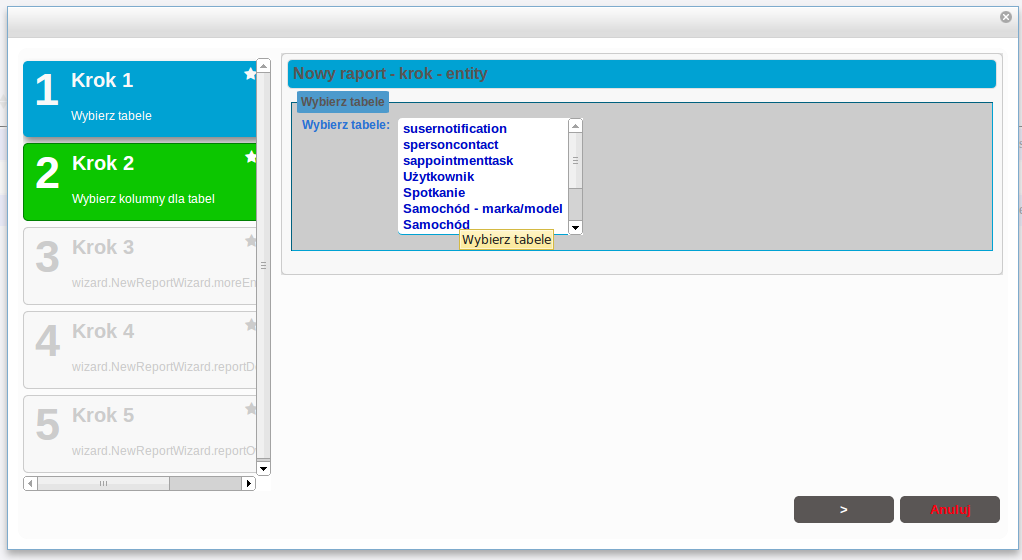
\includegraphics[width=1.0\textwidth]{images/rbuilder_step1}
		\caption[Kreator nowego raportu - krok 1]{
			Kreator nowego raportu - krok 1
		}
		\label{app:wizard_newReport_step1}
	\end{figure}	
	\begin{figure}[H]
		\centering
		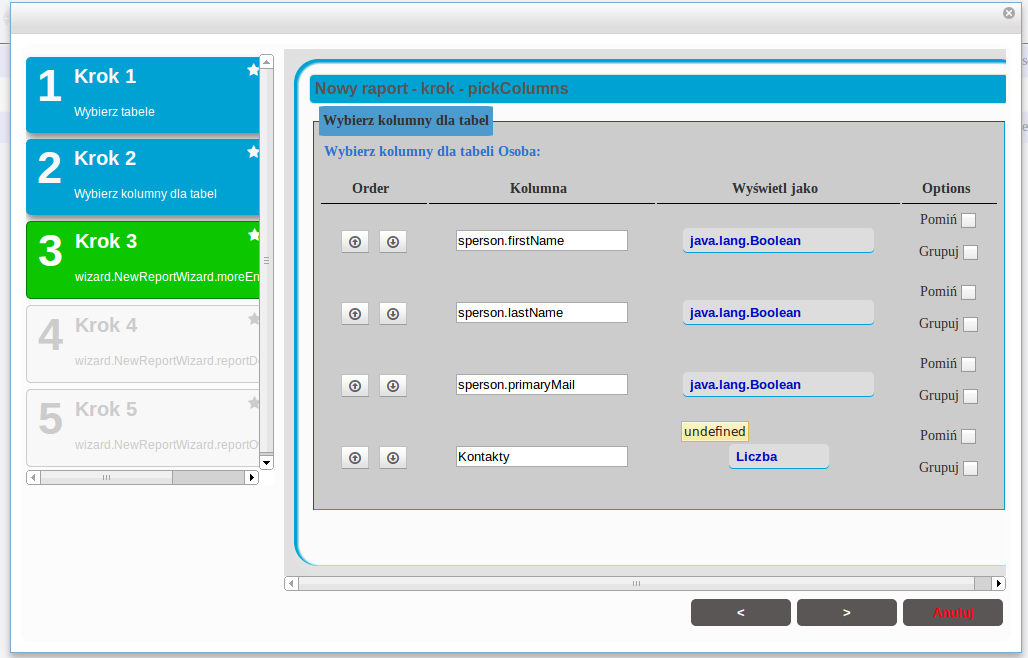
\includegraphics[width=1.0\textwidth]{images/rbuilder_step2}
		\caption[Kreator nowego raportu - krok 2]{
			Kreator nowego raportu - krok 2
		}
		\label{app:wizard_newReport_step2}
	\end{figure}		
	\begin{figure}[H]
		\centering
		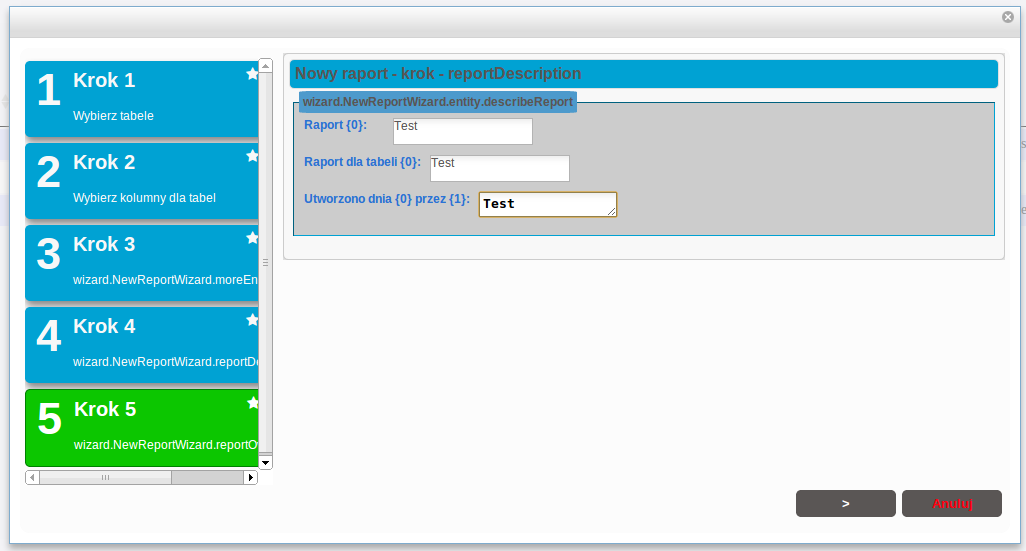
\includegraphics[width=1.0\textwidth]{images/rbuilder_step3}
		\caption[Kreator nowego raportu - krok 3]{
			Kreator nowego raportu - krok 3
		}
		\label{app:wizard_newReport_step2}
	\end{figure}	
	
	\begin{wrapfigure}{r}{0.5\textwidth}
		\centering
		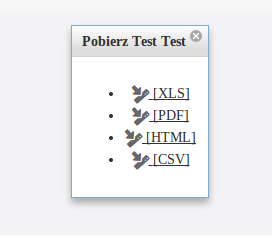
\includegraphics[width=1.0\textwidth]{images/rbuilder_generateReport}
		\caption[Generowanie nowego raportu - wybór docelowego formatu]{
			Generowanie nowego raportu - wybór docelowego formatu: \textbf{PDF}, \textbf{XLS}, \textbf{CSV}, \textbf{HTML}
		}
		\vspace{-10pt}
		\label{app:wizard_newReport_generateReport}
	\end{wrapfigure}
	
	Dzięki możliwości wykonywania akcji na poszczególnych wierszach tabeli, udało się przypisać dla każdego raportu link uruchamiający jego
	generowania oraz usunięcie. Usunięcie jest operacją trywialną z punktu widzenia użytkownika, ponieważ nie widzi on niczego poza 
	końcowym rezultatem. Z drugiej strony w momencie kliknięcia na przycisk \textbf{Generuj}, użytkownik ma możliwość
	wybrania końcowego formatu w jakim chciałby zobaczyć swoje dane. 
	Dalsza część funkcjonalności, czyli faktycznego zrenderowania gotowych danych została zaimplementowana z użyciem biblioteki wspierającej
	\textbf{JasperReports}, pochodzącą ze szkieletu aplikacji \textbf{Spring}. Przykładowy raport wygląda w następujący sposób:
	\begin{figure}[H]
		\centering
		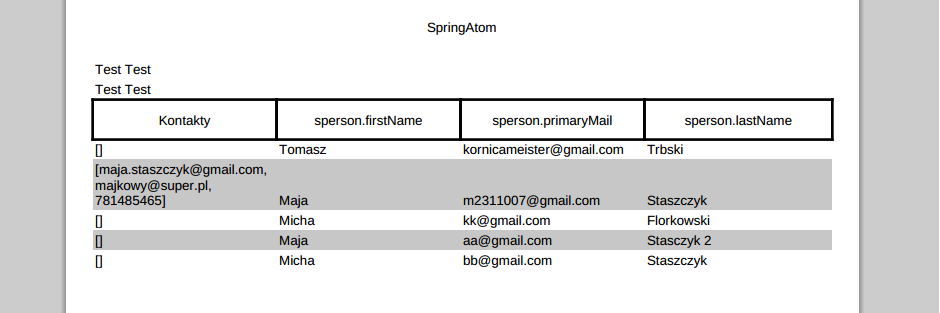
\includegraphics[width=1.0\textwidth]{images/rbuilder_report}
		\caption[Gotowy raport utworzony przez komponent \textbf{RBuilder}]{
			Gotowy raport utworzony przez komponent \textbf{RBuilder}
		}
		\label{app:wizard_newReport_report}
	\end{figure}		

\pagebreak
\subsubsection{Kreator nowego użytkownika}
	Kreator nowego użytkownika pozwala na tworzenie nowy obiektów klasy \textbf{SUser}. Kwestia uprawnień jest tutaj szczególnie ważna z uwagi na to, że w przewodniku wybierany jest zestaw ról. Role, do których przypisany jest użytkownik, stanowią późniejszą bazę do weryfikacji dostępności funkcji systemu dla poszczególnych użytkowników. 
	\begin{figure}[H]
		\centering
		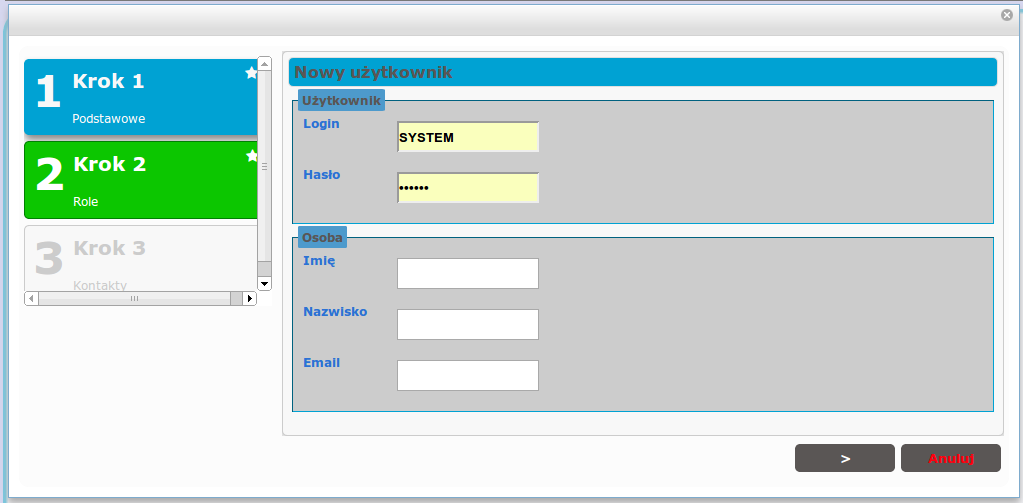
\includegraphics[width=1.0\textwidth]{images/newUser-basic}
		\caption[Kreator nowego użytkownika - dane podstawowe]{
			Kreator nowego użytkownika - dane podstawowe	
		}
		\label{app:newUser_basic}
	\end{figure}	
	\begin{figure}[H]
		\centering
		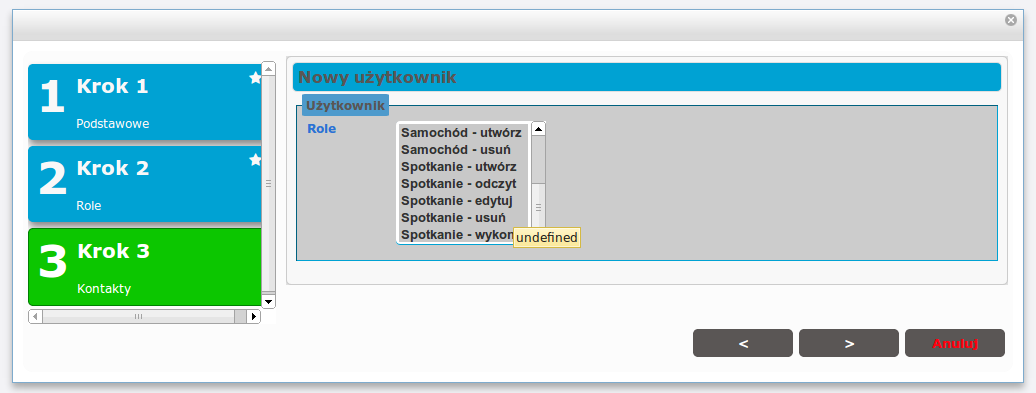
\includegraphics[width=1.0\textwidth]{images/newUser-roles}
		\caption[Kreator nowego użytkownika - uprawnienia użytkownika]{
			Kreator nowego użytkownika - uprawnienia użytkownika
		}
		\label{app:newUser_roles}
	\end{figure}	
	\begin{figure}[H]
		\centering
		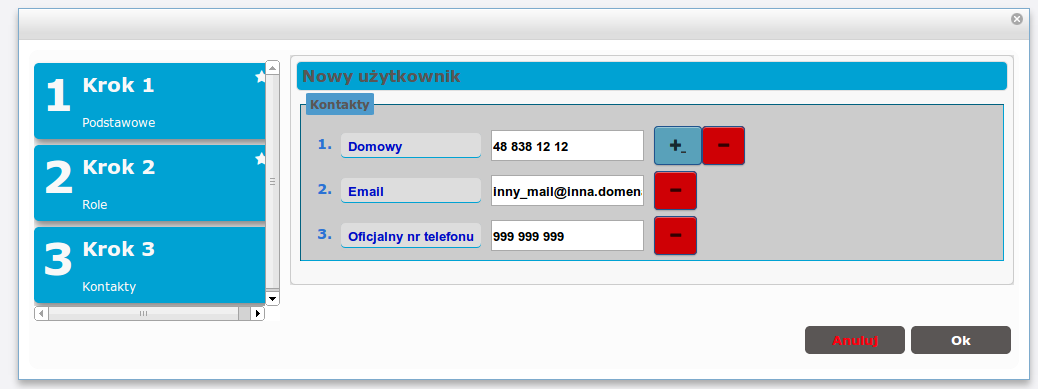
\includegraphics[width=1.0\textwidth]{images/newUser-contacts}
		\caption[Kreator nowego użytkownika - dane kontaktowe]{
			Kreator nowego użytkownika - dane kontaktowe
		}
		\label{app:newUser_contacts}
	\end{figure}	

\subsubsection{Kreator nowego samochodu}
	Kreator nowego samochodu został zaprojektowany aby tworzyć nowe obiekty klasy \textbf{SCar}.	Pierwszym krokiem jest podanie \textbf{numeru VIN}, z którego system odczytuje wszelkie możliwe dane, które można odkodować korzystając z informacji dostępnych publicznie. Na obecną chwilę są to:
	\begin{itemize}
		\item rok produkcji, zwracany jako lista lat w których samochód mógł być wyprodukowany,
		\item kraj, w którym samochód został wyprodukowany.
	\end{itemize}
	
	W drugim kroku kreator nowego samochodu podaje takie informacje jak:
	\begin{itemize}
		\item markę oraz model,
		\item numer tablicy rejestracyjnej,
		\item rok produkcji,
		\item rodzaj paliwa,
		\item właściciela.
	\end{itemize}
	\begin{figure}[H]
		\centering
		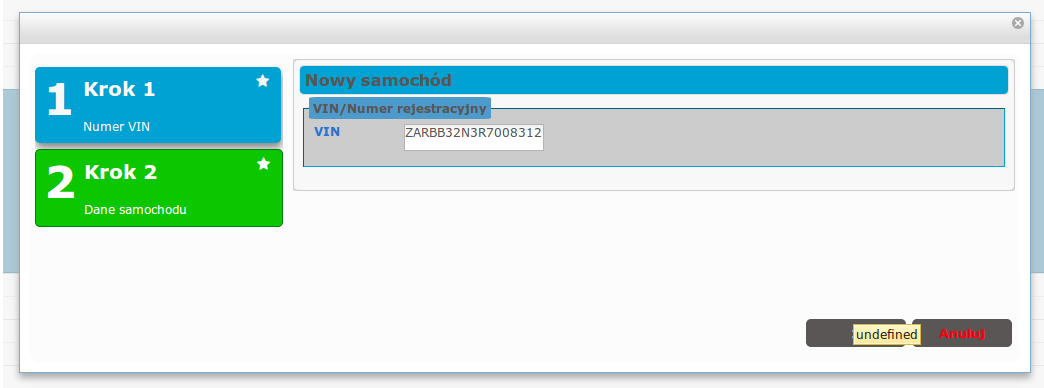
\includegraphics[width=1.0\textwidth]{images/newCar-vin}
		\caption[Kreator nowego samochodu - numer VIN]{
			Kreator nowego samochodu - numer VIN
		}
		\label{app:newCar_vin}
	\end{figure}	
	\begin{figure}[H]
		\centering
		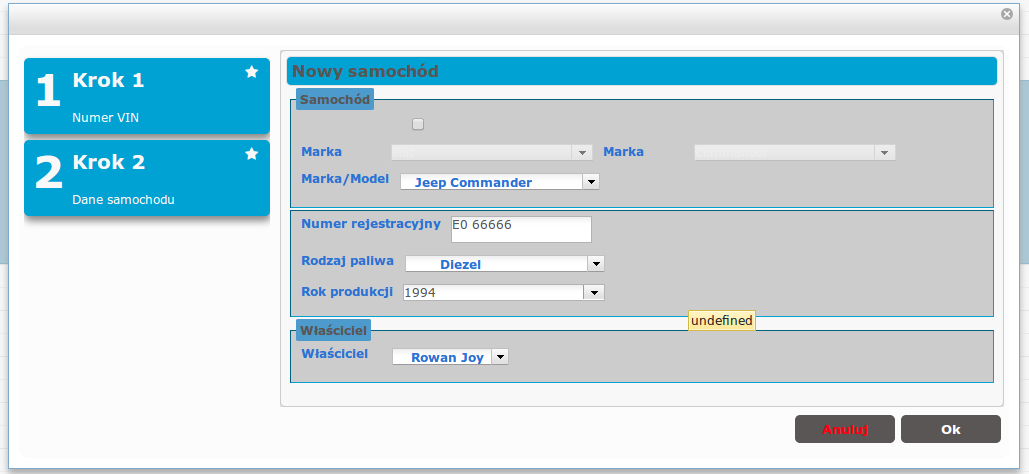
\includegraphics[width=1.0\textwidth]{images/newCar-data}
		\caption[Kreator nowego samochodu - pozostałe dane]{
			Kreator nowego samochodu - pozostałe dane
		}
		\label{app:newCar_data}
	\end{figure}

\subsubsection{Organizator spotkań}
	Organizator spotkań jest komponentem wspierającym zarządzania tym typem obiektów. 
	Pozwala na wgląd w listę wszystkich spotkań na 4 rożne sposoby:
	\begin{itemize}
		\item widok w kontekście wybranego dnia,
		\item widok w kontekście wybranego tygodnia,
		\item widok w kontekście wybranego miesiąca,
		\item widok tabelaryczny wszystkich spotkań.
	\end{itemize}
	
	\begin{figure}[H]
		\centering
		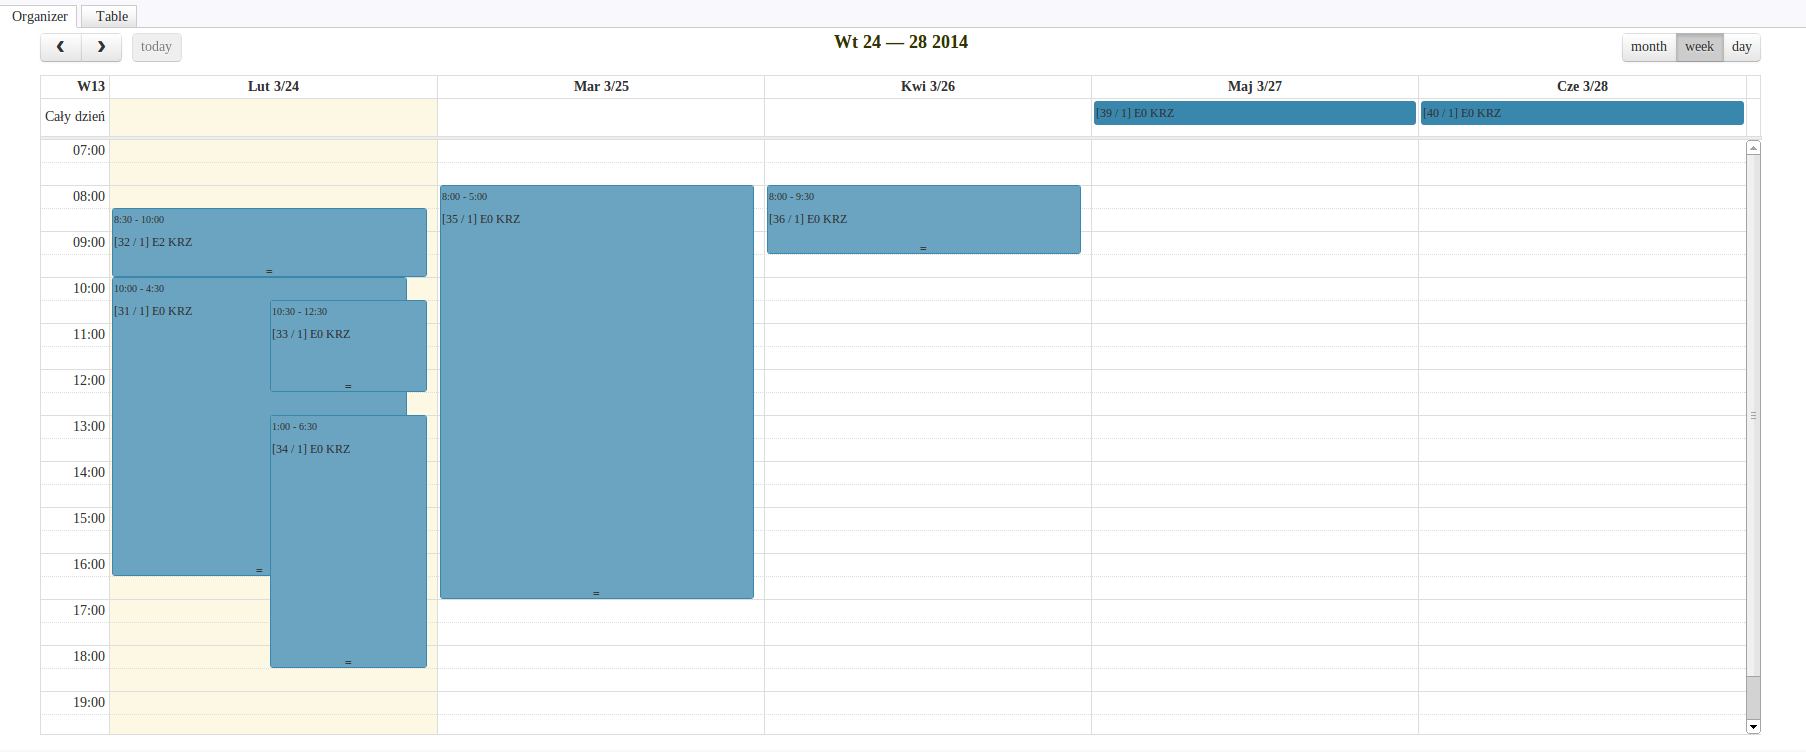
\includegraphics[width=1.0\textwidth]{images/calendarComponent-organizer}
		\caption[Komponent kalendarza wspierający organizację spotkań - organizer]{
			Komponent kalendarza wspierający organizację spotkań - organizer		
		}
		\label{app:component_calendar_organizer}
	\end{figure}	
	\begin{figure}[H]
		\centering
		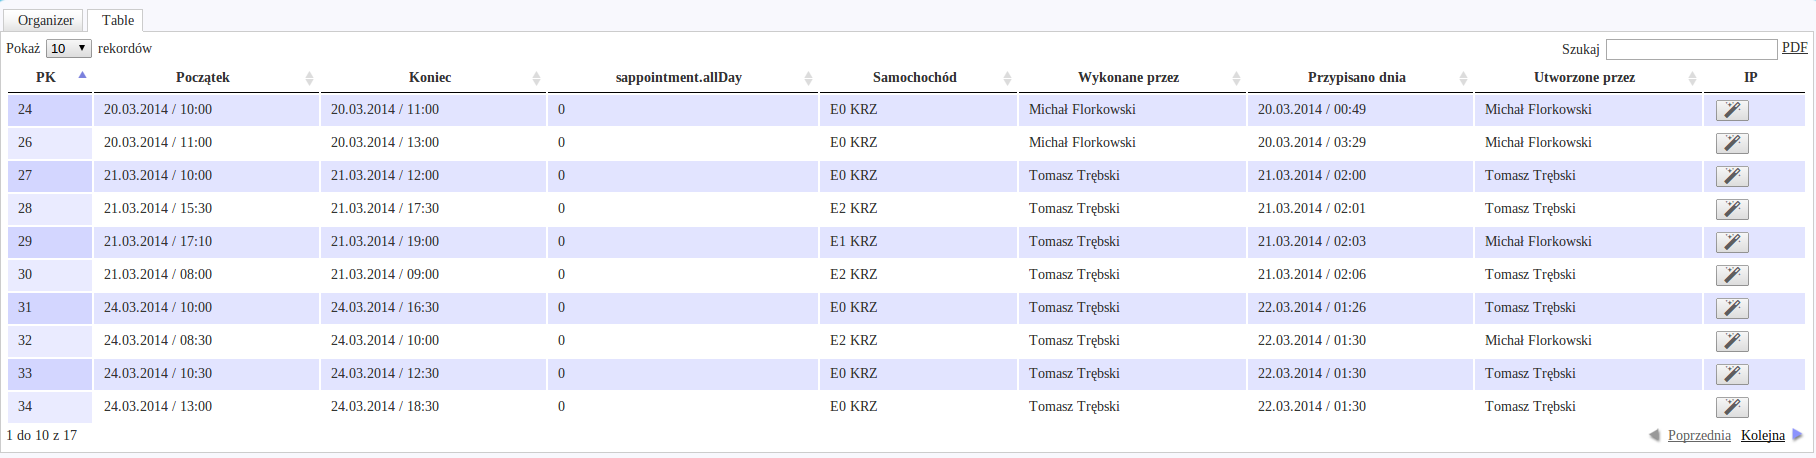
\includegraphics[width=1.0\textwidth]{images/calendarComponent-table}
		\caption[Komponent kalendarza wspierający organizację spotkań - tabela]{
			Komponent kalendarza wspierający organizację spotkań - tabela	
		}
		\label{app:component_calendar_table}
	\end{figure}	
	
	Z poziomu organizera możliwe jest natomiast otwarcie strony domenowej dla wybranego spotkania, dostarczającej znacznie więcej informacji niż sam organizator oraz uruchomienie przewodnika utworzenia nowego spotkania. Ważną cechą tego przewodnika jest to, że zakres dat wybrany w organizatorze jest zachowany. Sam kreator został napisany w oparciu o technologię \textbf{Spring Web Flow}, dzięki czemu na poziomie jednego komponentu można wprowadzić dane takie jak: 
	\begin{itemize}
		\item mechanik, który będzie odpowiedzialny za wizytę,
		\item mechanik raportujący dane spotkanie, niemniej taką możliwość posiadają jedynie osoby uprawnione do tego,
		\item wybrany samochód,
		\item lista zadań do wykonania podczas wizyty,
		\item opcjonalny komentarz dla wizyty.
	\end{itemize}
	
	\begin{figure}[H]
		\centering
		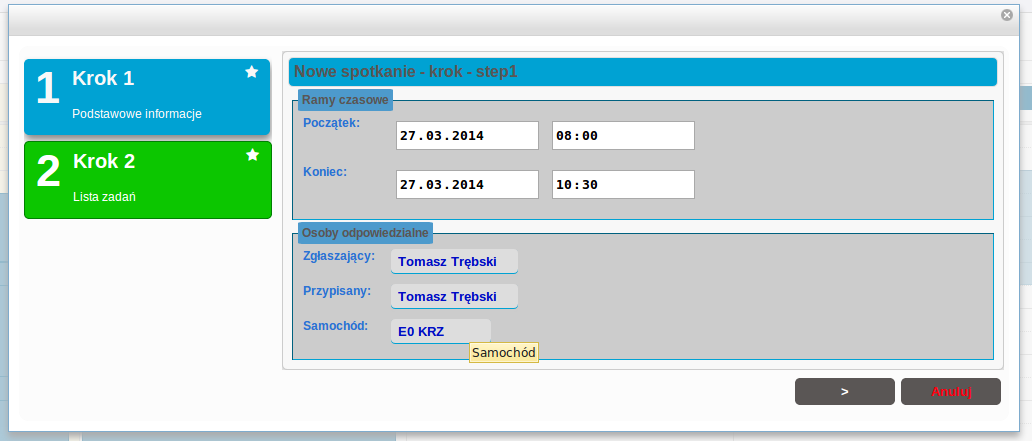
\includegraphics[width=1.0\textwidth]{images/newAppointment_step1}
		\caption[Kreator nowego spotkania - krok 1]{
			Kreator nowego spotkania - krok 1
		}
		\label{app:wizard_newAppointment_step1}
	\end{figure}
	\begin{figure}[H]
		\centering
		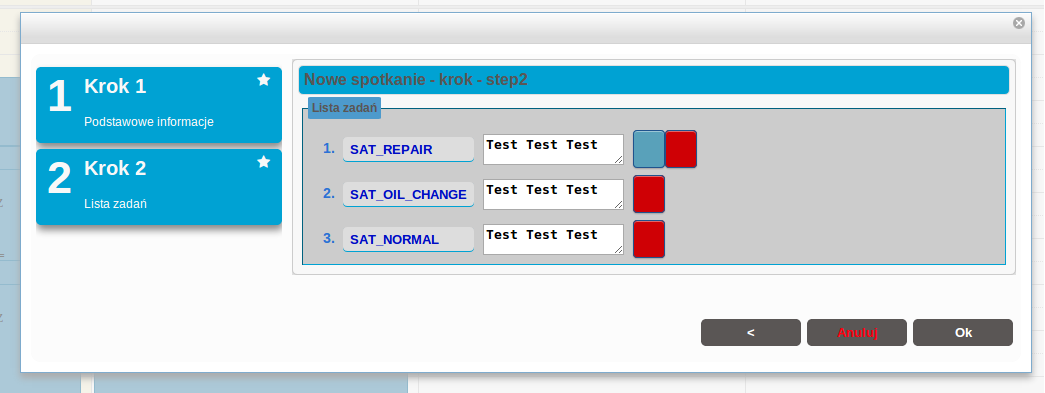
\includegraphics[width=1.0\textwidth]{images/newAppointment_step2}
		\caption[Kreator nowego spotkania - krok 2]{
			Kreator nowego spotkania - krok 2
		}
		\label{app:wizard_newAppointment_step2}
	\end{figure}
	\begin{figure}[H]
		\centering
		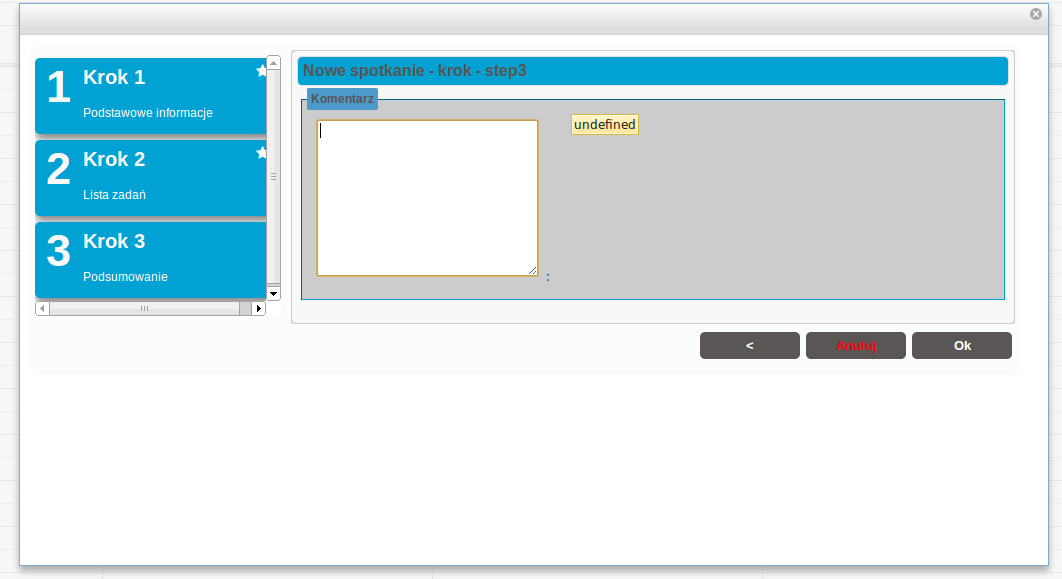
\includegraphics[width=1.0\textwidth]{images/newAppointment_step3}
		\caption[Kreator nowego spotkania - krok 3]{
			Kreator nowego spotkania - krok 3
		}
		\label{app:wizard_newAppointment_step3}
	\end{figure}		
	
	Dane wejściowe są walidowane pod kątem logiki biznesowej:
	\begin{itemize}
		\item termin spotkania:
		\begin{itemize}
			\item podane godziny (oraz czas) muszą mieścić się w wybranym zakresie [7-21],
			\item koniec spotkania nie może nastąpić później niż jego początek,
			\item zbyt krótkie (30 minut) oraz zbyt długie (10 dni),
			\item pokrywa się z co najmniej jednym spotkaniem dla mechanika wybranego jako wykonawca
		\end{itemize} 
		\item wybrany samochód:
		\begin{itemize}
			\item jeśli z właścicielem samochodu powiązane są jakiekolwiek problematyczne informacje, wyświetlane jest ostrzeżenie
		\end{itemize}
	\end{itemize}
	\pagebreak	
	\subsection{Architektura MVC} 								\subsection{Model - Warstwa danych}
		Na warstwę modelu danych składają się klasy, zwane dalej obiektami domenowymi. Zdefiniowane w aplikacji praktycznej klasy, należące do tej warstwy, opisują obiekty rzeczywiste, związane ze specyfikacją działalności warsztatu samochodowego, a także takie, dzięki którym możliwe jest zarządzanie użytkownikami aplikacji oraz ich uprawnieniami. 
		
		W wybranych przypadkach (tabela \ref{app:model_list_of}), obiekty domenowe są wersjonowane. Oznacza to, że \textbf{Hibernate} trzyma historię zmian w bazie danych. Modyfikacja każdego lub jedynie wybranych pól (jest to zależne od konfiguracji danego obiektu domenowego), powoduje nie tyle zapisywanie zmian do bazy, co utworzenie nowych rekordów w tabelach:
	\begin{itemize}
		\item \textbf{revinfo} - zawiera następujące kolumny:
		\begin{itemize}
			\item datę utworzenia rewizji,
			\item login użytkownika, który dokonał zmiany,
		\end{itemize} 
		\item \textbf{revchanges} - zawiera następujące kolumny:
		\begin{itemize}
			\item numer rewizji,
			\item nazwę (pełna nazwa klasy) modelu,
		\end{itemize}
		\item \textbf{\{nazwa\_tabeli\}\_history} - zawiera ona te pola, które zostały wybrane, co powoduje utworzenie nowej rewizji obiektu domenowego.
	\end{itemize}
	
	Aby wskazać konkretny obiekt domenowy, dla którego wymagana jest wiedza o historii jego modyfikacji, należy użyć adnotacji \textbf{@Audited}. Jeśli zostanie nią opatrzona cała klasa, będzie to równoznaczne z tym, że wszystkie atrybuty tej klasy będą kandydatami do utworzenia nowej rewizji. Z drugiej strony możliwe jest podanie jedynie konkretnych pól. Fragment klasy \textbf{SCar} (listing \ref{app:scar_version}) pokazuje użycie adnotacji nad polem \textbf{licencePlate}. 
	\begin{code}
		\inputminted[
			linenos=true,
			firstline=61,
			lastline=65,
			fontfamily=monospace,
			obeytabs=true,
			samepage=true,
			fontsize=\scriptsize
		]{java}{../SpringAtom_thesis/src/main/java/org/agatom/springatom/server/model/beans/car/SCar.java}
		% src file used
		\caption[Użycie adnotacji \textbf{@Audited}]{
			Użycie adnotacji \textbf{@Audited}, źródło: opracowanie własne
		}
		\label{app:scar_version}
	\end{code}
	
	\begin{center}
		\begin{longtable}{| p{4cm} | p{2cm} | p{8cm} |}
			\caption[Lista obiektów domenowych]{Lista obiektów domenowych \label{app:model_list_of}}\tabularnewline	
			
			% header
			\hline
				\multicolumn{1}{|c|}{\textbf{Obiekt domenowy}} 		&
				\multicolumn{1}{|c|}{\textbf{Wersjonowany}} 			&
				\multicolumn{1}{|c|}{\textbf{Opis}} 					\\
			\hline
			\endfirsthead
			
			\multicolumn{2}{c}
			{{\bfseries \tablename\ \thetable{} -- kontynuacja...}} 	\\
			\hline
				\multicolumn{1}{|c|}{\textbf{Obiekt domenowy}} 		&
				\multicolumn{1}{|c|}{\textbf{Wersjonowany}} 			&
				\multicolumn{1}{|c|}{\textbf{Opis}} 					\\
			\hline
			\endhead
				
			\hline
				\multicolumn{3}{|r|}{{Następna strona...}} 			\\
			\hline
			\endfoot
	
			\hline
			\endlastfoot	
			% end of header
			
			% body starts her
			SAppointment 		& 
			Nie			 		&
			Pojedyncza wizyta danego pojazdu w warsztacie samochodowym, która wydarzyła się w konkretnym momencie czasu. Wizyta powiązana jest z konkretnym samochodem, będącym jej podmiotem oraz zawiera informacje 
			o osobie, która zarejestrowała zgłoszenie i była jego wykonawcą (mogą to być inne osoby), a także listę czynności, jakie należało wykonać.
			\hline
			SAppointmentTask 	& 
			Nie					&
			Pojedyncza czynność, wykonana podczas wizyty. Czynność opisana jest przez jej typ (może to być, na przykład, wymiana oleju) oraz komentarz (dla wymiany oleju może to być informacja o tym, jaki olej został wymieniony). 
			\hline
			SAppointmentIssue 	& 
			Nie					&
			Opisuje problemową sytuację, związaną z danym spotkaniem. Dla pojedynczej wizyty sytuacją wyjątkową może być fakt nieodbycia się spotkania, ponieważ klient warsztatu, do który należy pojazd (podmiot wizyty), nie stawił się
			na umówiony termin. Jednocześnie klasa \textbf{SAppointmentIssue} jest rozszerzeniem klasy \textbf{SIssue}, dziedziczy więc wszystkie jej atrybuty. 
			\hline
			SCarMaster 			&
			Nie					& 
			Zawiera informacje opisujące samochód, które nie zależą od jego konkretnej rewizji. Są to atrybuty takie jak marka, model, producent i kraj, z którego samochód pochodzi.
			\hline
			SCar 				&
			Tak 				& 
			Centralny obiekt domenowy systemu. Na jego opis składają się atrybuty zdefiniowane w klasie \textbf{SCarMaster}, a także numer rejestracyjny, numer VIN, rok produkcji, rodzaj spalanego paliwa. Pojedynczy samochód
			powiązany jest z użytkownikiem systemu, będącym tym samym jego właścicielem. Samochód jest wersjonowany, a atrybuty, których zmiana powoduje utworzenie nowej rewizji to: właściciel, numer rejestracyjny oraz rodzaj paliwa. 
			\hline
			SIssue 				&
		 	Nie 				&
		 	\textbf{SIssue} opisuje sytuację wyjątkową, związaną z użytkownikiem systemu. Pojedynczy obiekt tego typu opisany jest przez użytkownika systemu, który zgłosił problem oraz użytkownika będącego podmiotem
		 	problematycznej sytuacji. 
		 	\hline
			SPerson 			& 
			Tak 				& 
			Ten obiekt domenowy jest pojedynczą osobą w systemie. Obiekt tego typu nie jest tożsamy z użytkownikiem systemu. Atrybuty opisujące ten typ obiektu to: imię, nazwisko oraz dane kontaktowe. Zmiana któregokolwiek z tych	 atrybutów
			równoznaczna jest z utworzeniem nowej rewizji. 
			\hline
			SPersonContact 		&
			Nie 				&
			Obiekt tego typu odnosi się do danych kontaktowych, które związane są osobą. Taki obiekt opisany jest przez atrybut, który odnosi się do tego, czy jest to numer telefonu komórkowego lub email. Drugim atrybutem jest
			wartość danego kontaktu.
			\hline
			SReport 			&
			Nie					& 
			Obiekt będący częścią komponentu \textbf{RBuilder}. Dostarcza informacji o położeniu plików opisujących zarówno strukturę szablonu, jak i pomocnych w procesie generowania raportu.
			\hline
			SAuthority	 		&
			Nie					& 
			Obiekty tej klasy opisują uprawnienia jakie przypisane są pojedynczemu użytkowniki systemu. Dzięki nim możliwe jest kontrolowanie do jakich obszarów funkcjonalnych, pojedynczy użytkownik ma dostęp, a które
			rejony są dla niego niedostępne. 
			\hline
			SUser 				&
			Tak 				& 
			\textbf{SUser} jest faktycznym użytkownikiem aplikacji. Pojedynczy obiekt opisany jest przez: login, hasło, zestaw zmiennych logicznych pozwalających określić stan konta (konto nieaktywne, zablokowane lub nieważne). Rola użytkownika, to kim on jest w kontekście systemu, opisane jest przez zbiór uprawnień. Modyfikacja atrybutów odnoszących się do nazwy użytkownika lub hasła skutkuje utworzeniem nowej rewizji obiektu. 
			\hline
			SUserNotification 	& 
			Nie 				& 
			Powiadomienie jest wiadomością jaka jest wysyłana użytkowniki systemu. Składa się z treści wiadomości oraz daty jej wysłania. Dodatkowym atrybutem jest zmienna logiczna odnosząca się do faktu, czy adresat odczytał powiadomienie. 
		\end{longtable}
	\end{center}	
	
\subsection{Model - Warstwa repozytoriów}
	Repozytoria w aplikacji demonstracyjnej są niczym więcej jak jedynie zdefiniowanymi w odpowiedni sposób interfejsami. Odpowiedni sposób oznacza, że dla każdego z nich, pierwszym interfejsem w drzewie dziedziczenia jest \textbf{Repository}. Jest to kluczowe ponieważ w ten sposób szkielet aplikacji \textbf{Spring} rozpoznaje repozytoria podczas skanowania \textbf{classpath}. Programista jest zobowiązany jedynie, w przypadku chęci skorzystania, do utworzenia w swojej klasie pola typu tego interfejsu, a właściwa referencja do obiektu zostanie umieszczona poprzez \textbf{dependency injection}. Kod na listingu \ref{app:scarmaster_repo} pokazuję definicje repozytorium. 
	\begin{code}
		\inputminted[
			linenos=true,
			firstline=43,
			lastline=77,
			fontfamily=monospace,
			obeytabs=true,
			samepage=true,
			fontsize=\scriptsize
		]{java}{../SpringAtom_thesis/src/main/java/org/agatom/springatom/server/repository/repositories/car/SCarMasterRepository.java}
		% src file used
		\caption[\textbf{SCarMasterRepository} - interfejs repozytorium dla modelu \textbf{SCarMaster}]{
			\textbf{SCarMasterRepository} - interfejs repozytorium	 pokazujący użycie metod mapowanych
			na kwerendy oraz bardziej skomplikowanego zapytania z użyciem adnotacji \textbf{Query}, źródło: opracowanie własne
		}
		\label{app:scarmaster_repo}
	\end{code}
	 
	\paragraph{Rozszerzenie natywnej funkcjonalności repozytoriów} \hspace{0pt} \\
	Funkcjonalność repozytoriów dostarczona przez moduł \textbf{Spring Data JPA} (\ref{tech:spring_data_jpa}) została rozbudowana o kilka dodatkowych funkcji. Rozszerzenie dotyczyło operacji wykonywanych na obiektach wersjonowanych, a zdefiniowane zostało w klasie \textbf{SRepository}, widocznej na listingu \ref{app:srepository}. 	Dodatkowe funkcje pozwalają na wyszukiwanie obiektów domenowych według następujących kryteriów:
	\begin{itemize}
		\item konkretny klucz główny oraz konkretna rewizja (metoda \textbf{findInRevision(ID,N)}),
		\item konkretny klucz główny oraz konkretne rewizje (metoda \textbf{findInRevisions(ID,N...)}),
		\item konkretny klucz, gdzie modyfikacja nastąpiła w pewnym momencie czasu (metoda \textbf{findRevisions(ID,DateTime,TimeOperator)}),
		\item obliczenie ilości modyfikacji (metoda \textbf{countRevisions(ID)}
	\end{itemize}
	
	\begin{code}
		\inputminted[
			linenos=true,
			firstline=36,
			lastline=56,
			fontfamily=monospace,
			obeytabs=true,
			samepage=false,
			fontsize=\scriptsize
		]{java}{\SpringatomScrPath{/server/repository/SRepository.java}}
		% src file used
		\caption[\textbf{SRepository} - abstrakcyjne repozytorium wspierające dostęp do rewizji]{
			\textbf{SRepository} - abstrakcyjne repozytorium wspierające dostęp do rewizji, źródło: opracowanie własne
		}
		\label{app:srepository}
	\end{code}
	
	Uwzględnienie rozszerzenia nie byłoby możliwe bez modyfikacji procesu, podczas którego moduł \textbf{Spring Data JPA} tworzył obiekty implementujące funkcjonalność repozytoriów, zdefiniowaną poprzez interfejsy. Wprowadzony został dodatkowy element - fabryka, która nadpisywała oryginalny algorytm dostarczając implementacji zdefiniowanych w aplikacji praktycznej. Listing \ref{app:srepositories_factory_bean} pokazuje wycinek kodu klasy \textbf{SRepositoriesFactoryBean} realizujący tą czynność. 
	\begin{code}
		\inputminted[
			gobble=2,
			linenos=true,
			firstline=89,
			lastline=105,
			fontfamily=monospace,
			obeytabs=true,
			samepage=false,
			fontsize=\scriptsize
		]{java}{\SpringatomScrPath{/server/repository/factory/SRepositoriesFactoryBean.java}}
		\caption[\textbf{SRepositoriesFactoryBean} - fabryka repozytoriów dla implementacji własnej funkcjonalności]{
			\textbf{SRepositoriesFactoryBean} - fabryka repozytoriów dla implementacji własnej funkcjonalności, źródło: opracowanie własne
		}
		\label{app:srepositories_factory_bean}
	\end{code}
	
	\clearpage
	\paragraph{Lista repozytoriów} \hspace{0pt} \\
	Poniższa tabela zawiera listę repozytoriów zdefiniowanych w aplikacji demonstracyjnej, nazwę odpowiadającego jej obiektu domenowego oraz informację o tym, czy repozytorium wspiera dostęp do dziennika zmian tego obiektu.
	\begin{center}
		\begin{longtable}{| p{6cm} | p{5cm} | p{2cm} |}
			\caption[Lista repozytoriów danych]{Lista repozytoriów danych \label{mvc:repo_list}}\tabularnewline	
			
			% header
			\hline
				\multicolumn{1}{|c|}{\textbf{Repozytorium}} 			&
				\multicolumn{1}{|c|}{\textbf{Obiekt domenowy}} 		&
				\multicolumn{1}{|c|}{\textbf{Dziennik zmian}} 			\\
			\hline
			\endfirsthead
			
			\multicolumn{2}{c}
			{{\bfseries \tablename\ \thetable{} -- kontynuacja...}} 	\\
			\hline
				\multicolumn{1}{|c|}{\textbf{Repozytorium}} 			&
				\multicolumn{1}{|c|}{\textbf{Obiekt domenowy}} 		&
				\multicolumn{1}{|c|}{\textbf{Dziennik zmian}} 			\\
			\hline
			\endhead
				
			\hline
				\multicolumn{4}{|r|}{{Następna strona...}} \tabularnewline
			\hline
			\endfoot
	
			\hline
			\endlastfoot	
			% end of header
			
			% body starts her
			SAppointmentRepository & SAppointment & Nie \hline
			SAppointmentIssueRepository & SAppointmentIssue & Nie \hline
			SAppointmentTaskRepository & SAppointmentTask & Nie \hline
			SCarMasterRepository & SCarMaster & Nie \hline
			SCarRepository & SCar & Tak \hline
			SIssueRepository & SIssue & Nie \hline
			SPersonContactRepository & SPersonContacat & Nie \hline
			SPersonRepository & SPerson & Tak \hline
			SReportRepository & SReport & Tak \hline
			SUserAuthorityRepository & SUserAuthority & Nie \hline
			SUserNotificationRepository & SUserNotification & Nie \hline
			SUserRepository & SUser & Tak
		\end{longtable}
	\end{center}	
	
\subsection{Model - Warstwa serwisów}
	Serwisy	stanowią w aplikacji element realizujący logikę biznesową, jednak nie odnoszą się one jedynie do operacji
	na modelu danych. Również inne moduły aplikacji korzystają z własnych serwisów, jako miejsc gdzie funkcjonalność została
	zebrana i jest gotowa do użycia. 	
	\begin{code}
		\inputminted[
			linenos=true,
			firstline=33,
			lastline=45,
			fontfamily=monospace,
			obeytabs=true,
			samepage=false,
			fontsize=\scriptsize
		]{java}{\SpringatomScrPath{/server/service/domain/SPersonService.java}}
		% src file used
		\caption[\textbf{SPersonService} - interfejs serwisu dla modelu \textsc{SPerson}]{
			\textbf{SPersonService} - interfejs serwisu dla modelu \textsc{SPerson}, źródło: opracowanie własne
		}
		\label{app:sperson_service}
	\end{code}
	
	Serwisy zostały zaprojektowane aby korzystać z repozytoriów danych. Ma to swoje pozytywne skutki
	i nie jest wcale oznaką nadmiarowości kodu, czy też jego duplikowania. Z uwagi na fakt, ze serwisy
	odwołują się do danych poprzez interfejsy repozytoriów, podnosi to znacząco możliwości 
	późniejszych zmian w postaci silnika bazy danych. Dodatkową korzyścią jest zwiększenie możliwości testowania
	interesujących funkcji bez konieczności posiadania działającego połączenia z bazą danych.
	
\subsection{Widok - Warstwa widoku}
	Warstwa widoku została zaprojektowana z wykorzystaniem standardowej biblioteki tagów \textbf{JSTL}, plików \textbf{JSP} oraz biblioteki \textbf{Apache Tiles} \ref{tech:tiles}. Dzięki \textbf{Tiles} udało się zminimalizować zbędny kod w plikach \textbf{JSP} definiujący elementy, takie jak nagłówek strony, element \textit{<head>}. Do gotowego widoku można się było następnie odwoływać po unikatowej nazwie. 
	\begin{code}
		\inputminted[
			linenos=true,
			firstline=23,
			lastline=36,
			fontfamily=monospace,
			obeytabs=true,
			samepage=true,
			fontsize=\scriptsize
		]{xml}{../SpringAtom_thesis/src/main/webapp/ui/core/core-page-view.xml}
		% src file used
		\caption[Definicja \textit{tile} - podstawowego elementu widoku]{
			Definicja \textit{tile} - podstawowy element widoku w rozumieniu technologi Apache Tiles, źródło: opracowanie własne		
		}
		\label{app:apache_tiles_example}
	\end{code} 
	
	Listing \ref{app:apache_tiles_example} pokazuje deklarację abstrakcyjnej \textit{płytki}. Abstrakcyjność jest tutaj kwestią umowną ponieważ
	można by tę \textit{płytkę} zwrócić z dowolnego kontrolera i została by ona zrenderowana do poprawnego widoku HTML. Elementem, który jest w tej definicji
	zadeklarowany, lecz nie zdefiniowany, jest \textit{content} - faktyczna zawartość danej strony. Mimo to plik \textbf{JSP} odpowiadający tej płytce
	zawiera kod, który umieści ją w ostatecznej strukturze DOM. 
	
	\begin{code}
		\inputminted[
			linenos=true,
			firstline=51,
			lastline=53,
			fontfamily=monospace,
			obeytabs=true,
			samepage=true,
			fontsize=\scriptsize
		]{jsp}{../SpringAtom_thesis/src/main/webapp/ui/core/page.jsp}
		% src file used
		\label{app:apache_tiles_example_jsp}
		\caption[Fragment pliku \textbf{JSP} umieszczający w nim atrybut \textbf{content}]{
			Fragment pliku \textbf{JSP} umieszczający w nim atrybut \textbf{content}, źródło: opracowanie własne
		}
	\end{code}
	
	\paragraph{Generyczny kontroler zwracający widok} \hspace{0pt} \\
	Aby zminimalizować ilość kodu i pisania kontrolera posiadającego metody zwracające nazwy widoków dla każdego możliwego adresu, w aplikacji praktycznej istnieje tylko jeden kontroler wspierający to zadania. \textbf{SVTilesViewControler} działa w oparciu o plik, zawierający wpisy opisujące mapowania adresów na nazwy widoków. Adres jest tutaj kluczem, z którego kontroler buduje obiekt klasy \textbf{UriTemplate}. \textbf{UriTemplate} działa podobnie do wyrażenia regularnego i pozwala na stwierdzenie, czy adres pobrany z żądania, pasuje do szablonu. Listing \ref{app:svTilesViewController} pokazuje definicję metody realizującej mapowanie, natomiast listing \ref{app:mapping_props} to lista adresów wraz z odpowiadającymi im widokami.
	\begin{code}
		\inputminted[
			linenos=true,
			firstline=50,
			lastline=61,
			fontfamily=monospace,
			obeytabs=true,
			samepage=true,
			fontsize=\scriptsize
		]{java}{\SpringatomScrPath{/webmvc/controllers/SVTilesViewController.java}}
		% src file used
		\caption[Generyczny kontroler zwracający nazwy widoków]{
			Generyczny kontroler zwracający nazwy widoków zdefiniowanych w pliku \ref{app:mapping_props}, źródło: opracowanie własne
		}
		\label{app:svTilesViewController}
	}
	\end{code}
		\begin{code}
		\inputminted[
			linenos=true,
			firstline=18,
			lastline=34,
			fontfamily=monospace,
			obeytabs=true,
			samepage=true,
			fontsize=\scriptsize
		]{properties}{../SpringAtom_thesis/src/main/resources/org/agatom/springatom/webmvc/url-mapping.properties}
		% src file used
		\caption[Mapowania adresów na nazwy widoków]{
			Mapowania adresów na nazwy widoków, źródło: opracowanie własne
		}
		\label{app:mapping_props}
	\end{code}
		 
\subsection{Globalna - Warstwa konwersji}
	Warstwa konwersji typów jest modułem \textbf{Spring}, który wykorzystywany jest w momencie, kiedy z obiektu typu A programista chce uzyskać obiekt typu B. Dobrym przykładem jest najczęściej moment, w którym w kodzie JSP umieszczamy bezpośrednio nasz obiekt, korzystając z biblioteki tagów dostarczonej przez \textbf{Spring}. W tym momencie uruchamiany jest proces, mający na celu konwersję obiektu do reprezentatywnej postaci łańcucha znakowego, który można będzie wkomponować do drzewa DOM. Jest to rozwiązanie efektywne, niemniej posiadające jedno uchybienie. W przypadku, gdy programista chciałby uzyskać selektywny sposób, zależny od kontekstu, w jakim znajduje się obiekt lub też chęci uzyskania wartości jednego z atrybutów, nie jest on w stanie osiągnąć zamierzonego rezultatu, z uwagi na sposób, w jaki działa konwersja typów. Znalezienie pierwszego konwertera, który jest w stanie przeprowadzić żądaną transformację kończy proces wyszukiwania. Nie oznacza to wcale, że uzyskany wynik będzie zgodny z oczekiwanym. Z tego powodu aplikacja demonstracyjna rozszerza istniejącą funkcjonalność przez umożliwienie wybiórczego konwertowania między poszczególnymi typami. Na obecną chwilę zostało to zaimplementowane dla obiektów domenowych, a klasą kontrolującą selektywny proces jest \textbf{PersistableConverterPicker}.
	\begin{code}
		\inputminted[
			linenos=true,
			firstline=51,
			lastline=69,
			fontfamily=monospace,
			obeytabs=true, 
			samepage=true,
			fontsize=\scriptsize
		]{java}{\SpringatomScrPath{/server/model/conversion/picker/PersistableConverterPicker.java}}
		\caption[\textbf{PersistableConverterPicker} - koordynator selektywnej konwersji typów]{
			\textbf{PersistableConverterPicker} - koordynator selektywnej konwersji typów, źródło: opracowanie własne
		}
		\label{app:conversion_persistableToString}
	\end{code}
	\textbf{PersistableConverterPicker} posiada metody które pozwalają na wybór selektywnego konwertera do wykonania operacji
	transformacji. Zostało również zapewnione wsparcie dla istniejącej funkcjonalności, bez użycia selektora. Ta część realizowana jest w 
	metodzie \textbf{getDefaultConverter(...)}.
	\begin{code}
		\inputminted[
			linenos=true,
			firstline=72,
			lastline=99,
			fontfamily=monospace,
			obeytabs=true, 
			samepage=true,
			fontsize=\scriptsize
		]{java}{\SpringatomScrPath{/server/model/conversion/picker/PersistableConverterPicker.java}}
		\caption[\textbf{PersistableConverterPicker} - pobranie domyślnego konwertera dla typu]{
			\textbf{PersistableConverterPicker} - pobranie domyślnego konwertera dla typu, źródło: opracowanie własne
		}
		\label{app:conversion_defaultConverter}
	\end{code}
	
	\clearpage
	Selektywne konwertery różnią się od normalnych jedynie użyciem specjalnej adnotacji \textbf{PersistableConverterUtility} (listing \ref{app:conversion_PersistableConverterUtility}), która pozwala na ustalenie, że:
	\begin{itemize}
		\item konwerter jest domyślny, jeśli nie został zdefiniowany klucz,
		\item konwerter jest selektywny, jeśli istnieje zdefiniowany klucz.
	\end{itemize}
	
	\begin{code}
		\inputminted[
			linenos=true,
			firstline=34,
			lastline=52,
			fontfamily=monospace,
			obeytabs=true, 
			samepage=true,
			fontsize=\scriptsize
		]{java}{\SpringatomScrPath{/server/model/conversion/annotation/PersistableConverterUtility.java}}
		\caption[\textbf{PersistableConverterUtility} - adnotacja opisująca selektywny konwerter]{
			\textbf{PersistableConverterUtility} - adnotacja opisująca selektywny konwerter
		}
		\label{app:conversion_PersistableConverterUtility}
	\end{code}

	\pagebreak	
	\subsection{Plany rozwojowe}								Aplikacja demonstracyjna jest obecnie na etapie dalszego rozwoju. Posiada szeroko zdefiniowane moduły zaprojektowane, aby wspierać takie
rejony jak:
\begin{itemize}
	\item generyczna warstwa operacji bazodanowych,
	\item warstwa logiki biznesowej udostępnionej przez serwisy,
	\item moduł komponentów dla budowy tabel oraz stron obiektów domenowych,
	\item selektywna warstwa konwersji,
	\item tagi oddelegowane dla przewodników opartych o Spring Web Flow,
	\item model danych wraz z jego abstrakcyjną warstwą (interfejsy) do użytku zewnętrznego,
	\item moduł obsługujący funkcjonalność raportowania.
\end{itemize}

W większości przypadków uzyskana funkcjonalność jest jednak na etapie implementacji i niektóre z niedopracowanych elementów 
ulegną zmianie, celem uproszczenia zarządzania złożonością projektu oraz usunięcia nadmiarowych klas, jak także słabo konfigurowalnych części.
Plany rozwojowe aplikacji zostały przedstawione w tabeli \ref{app:changes_in_future}.
\begin{center}
	\begin{longtable}{|l|p{10cm}|}
		\caption[Plany rozwojowe aplikacji demonstracyjnej]{
			Plany rozwojowe aplikacji demonstracyjnej
		}
		\label{app:changes_in_future}
		\tabularnewline	
		
		\hline
			\multicolumn{1}{|c|}{\textbf{Moduł}}		&
			\multicolumn{1}{|c|}{\textbf{Opis zmian}}	\tabularnewline
		\hline
		\endfirsthead
		
		\multicolumn{2}{c}
		{{\bfseries \tablename\ \thetable{} -- kontynuacja...}} \tabularnewline
		\hline
			\multicolumn{1}{|c|}{\textbf{Moduł}}		&
			\multicolumn{1}{|c|}{\textbf{Opis zmian}}	\tabularnewline
		\hline
		\endhead
			
		\hline
			\multicolumn{2}{|r|}{{Następna strona...}} \tabularnewline \hline
		\endfoot
		\hline
		\endlastfoot	
		
		\textbf{ComponentBuilder}	&
		Ogólne rozszerzenie i optymalizacja modułu \textbf{ComponentBuilder} dotyczyć będzie:
		\begin{itemize}
			\item wsparcie dla cache'owania raz załadowanych komponentów,
			\item przeniesienie definicji stron do deklaratywnego języka XML.
			Będzie to możliwe po usprawnieniu działania selektywnych konwerterów oraz 
			zwiększy możliwość zmian zgodnie z wymaganiami, bez konieczności zmian w plikach Java,
			\item przeniesienie kodu widoku stron domenowych do łatwiejszego w zarządzaniu oraz utrzymaniu kodu ExtJS,
			\item wprowadzenie automatycznego mechanizmu generującego przekierowania do stron obiektów domenowych,
			\item połączenie kontrolerów odpowiedzialnych za obsługę żądań pochodzących od komponentów typu \textbf{tabele} oraz \textbf{strony domenowe}. Celem tego działania jest ujednolicenie adresów sugerujące, że oba komponenty służą podobnemu celowi.
		\end{itemize}
		\hline		
		\textbf{WebFlow}			&
		Zaprojektowanie biblioteki wspierającej 
		funkcjonalność \textbf{Spring Web Flow} dla biblioteki ExtJS. Decyzja podyktowana jest 
		chęcią zminimalizowania użycia różnorodnych bibliotek JavaScript. Gotowa biblioteka
		byłaby udostępniona na licencji OpenSource.
		\hline
		\textbf{Selektywne konwertery}	&
		Rozszerzenie możliwości selektywnych konwerterów o obiekty inne niż domenowe oraz
		wsparcie dla możliwości definiowana powtarzających się selektorów - kluczy w kontekście
		globalnym, ale unikatowych w kontekście danego obiektu podlegającego konwersji.
		\hline
		\textbf{Kod ogólny}				&
		Usunięcie pozostałości nadmiarowego kodu, który pozostał po uaktualnieniu aplikacji,
		do korzystania z najnowszej wersji (4.0.0) szkieletu aplikacji \textbf{Spring}.
		\hline
		\textbf{Widok}					&
		Wsparcia dla ExtJS - migracja istniejących komponentów warstwy widoku użytkownika do 
		szkieletu aplikacji ExtJS. Prawdopodobnym wyborem będzie wykorzystanie ExtJS w wersji 4.x.x z uwagi
		na lepszą wydajność i większe możliwości biblioteki, w porównaniu do poprzednich wersji.
		\hline
		\textbf{RBuilder}			&
		Zrezygnowania z ciężkiego w użyciu oraz utrzymaniu sposobu generowania raportów w aplikacji poprzez
		bibliotekę \textbf{DynamicJasper}. Przeniesienie bezpośredniego generowania raportów do tabelek oraz
		inwestygacja możliwych technologii do wykorzystania w przypadku eksportowania raportu do formatów takich jak
		HTML, CSV, PDF oraz XLS.		
		\hline
		\textbf{Przewodniki}			&
		Ukończenie wszystkich wymaganych kreatorów służących zarówno do modyfikacji, jak i tworzenia nowych obiektów domenowych.
		\hline
		\textbf{Terminarz spotkań}		&
		Ukończenie prac nad terminarzem spotkań. Obecna funkcjonalność pozwala na tworzenie obiektów, które następnie
		można przeglądać z użyciem kalendarza (podobnego do używanego w programie Outlook). 	
		\hline
		\textbf{Dekodowane numeru VIN}		&
		Rozszerzenie obecnych możliwości dekodera numeru VIN o pobieranie informacji, takich jak:
		\begin{itemize}
			\item wytwórca samochodu,
			\item marka oraz model,
			\item typ nadwozia,
			\item typ paliwa,
			\item typ silnika
		\end{itemize}							
	\end{longtable}
\end{center}
		
\section{Diagramy UML, schemat bazy danych}  					\subsection{Schemat bazy danych}
\begin{figure}[H]
	\centering
	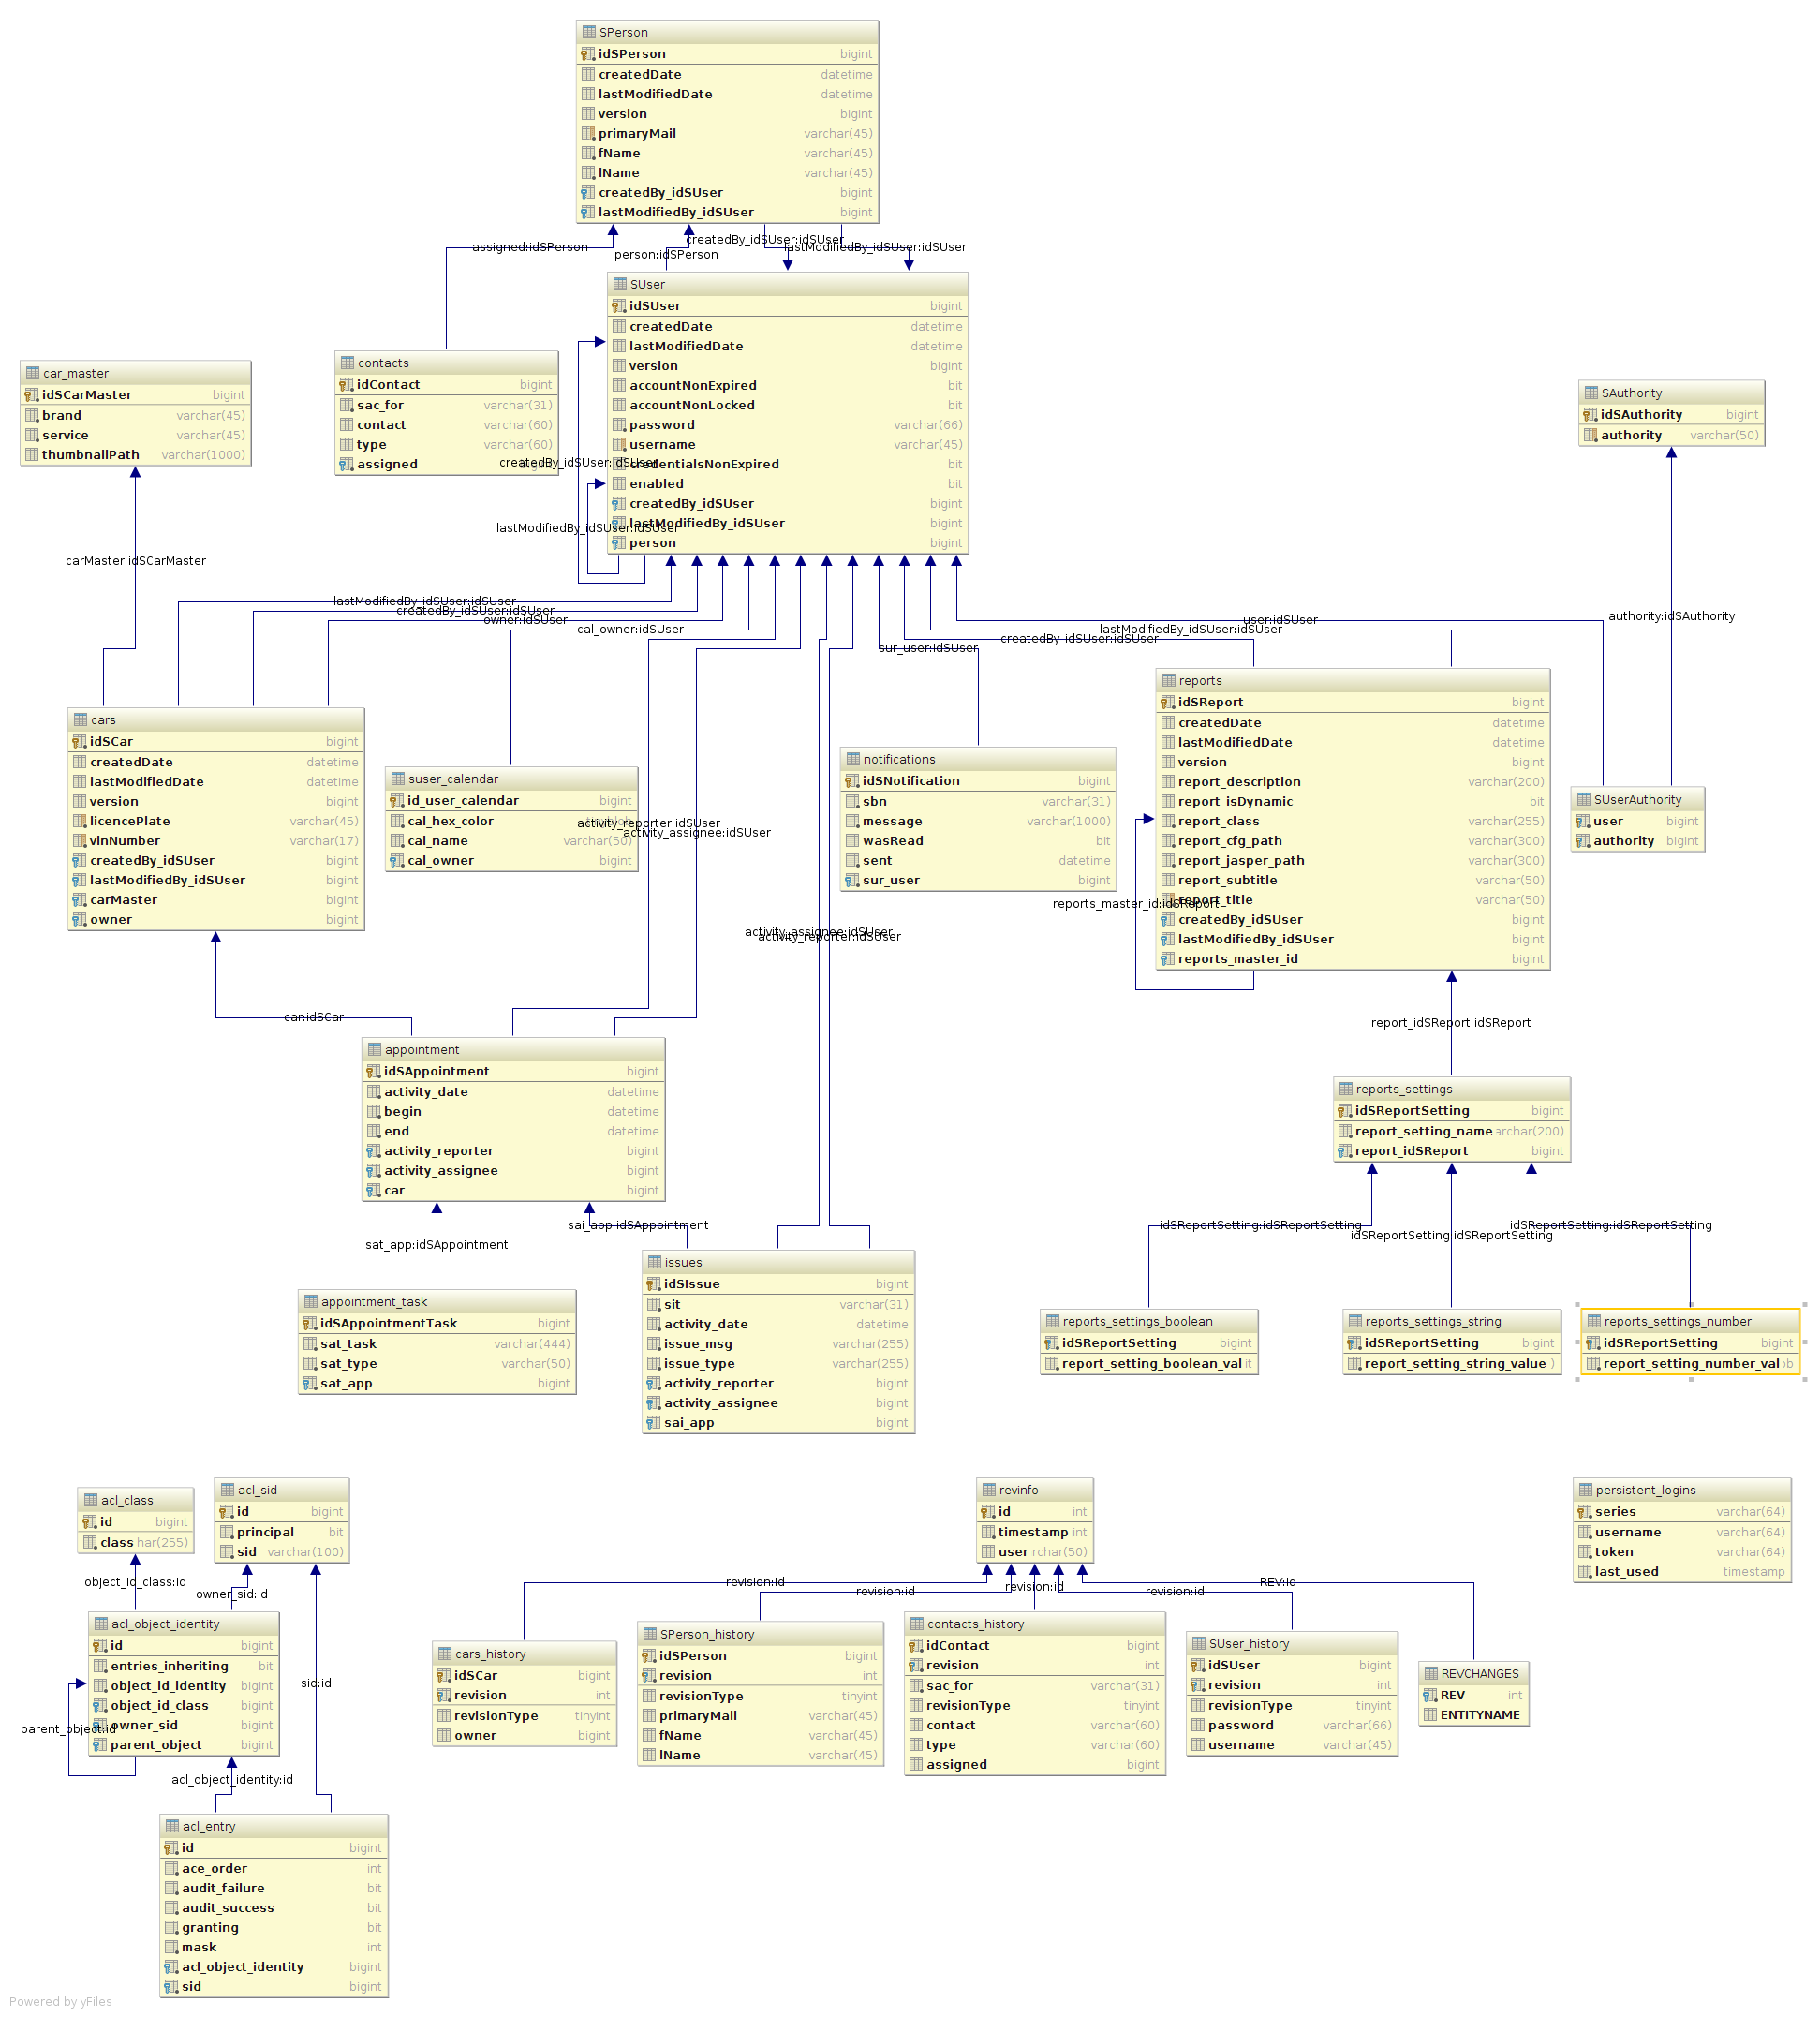
\includegraphics[width=1.1\textwidth]{images/db_UML}
	\caption[Schemat bazy danych aplikacji demonstracyjnej]{
		Schemat bazy danych aplikacji demonstracyjnej
	}
	\label{app:schema_db}
\end{figure}
\begin{figure}[H]
	\centering
	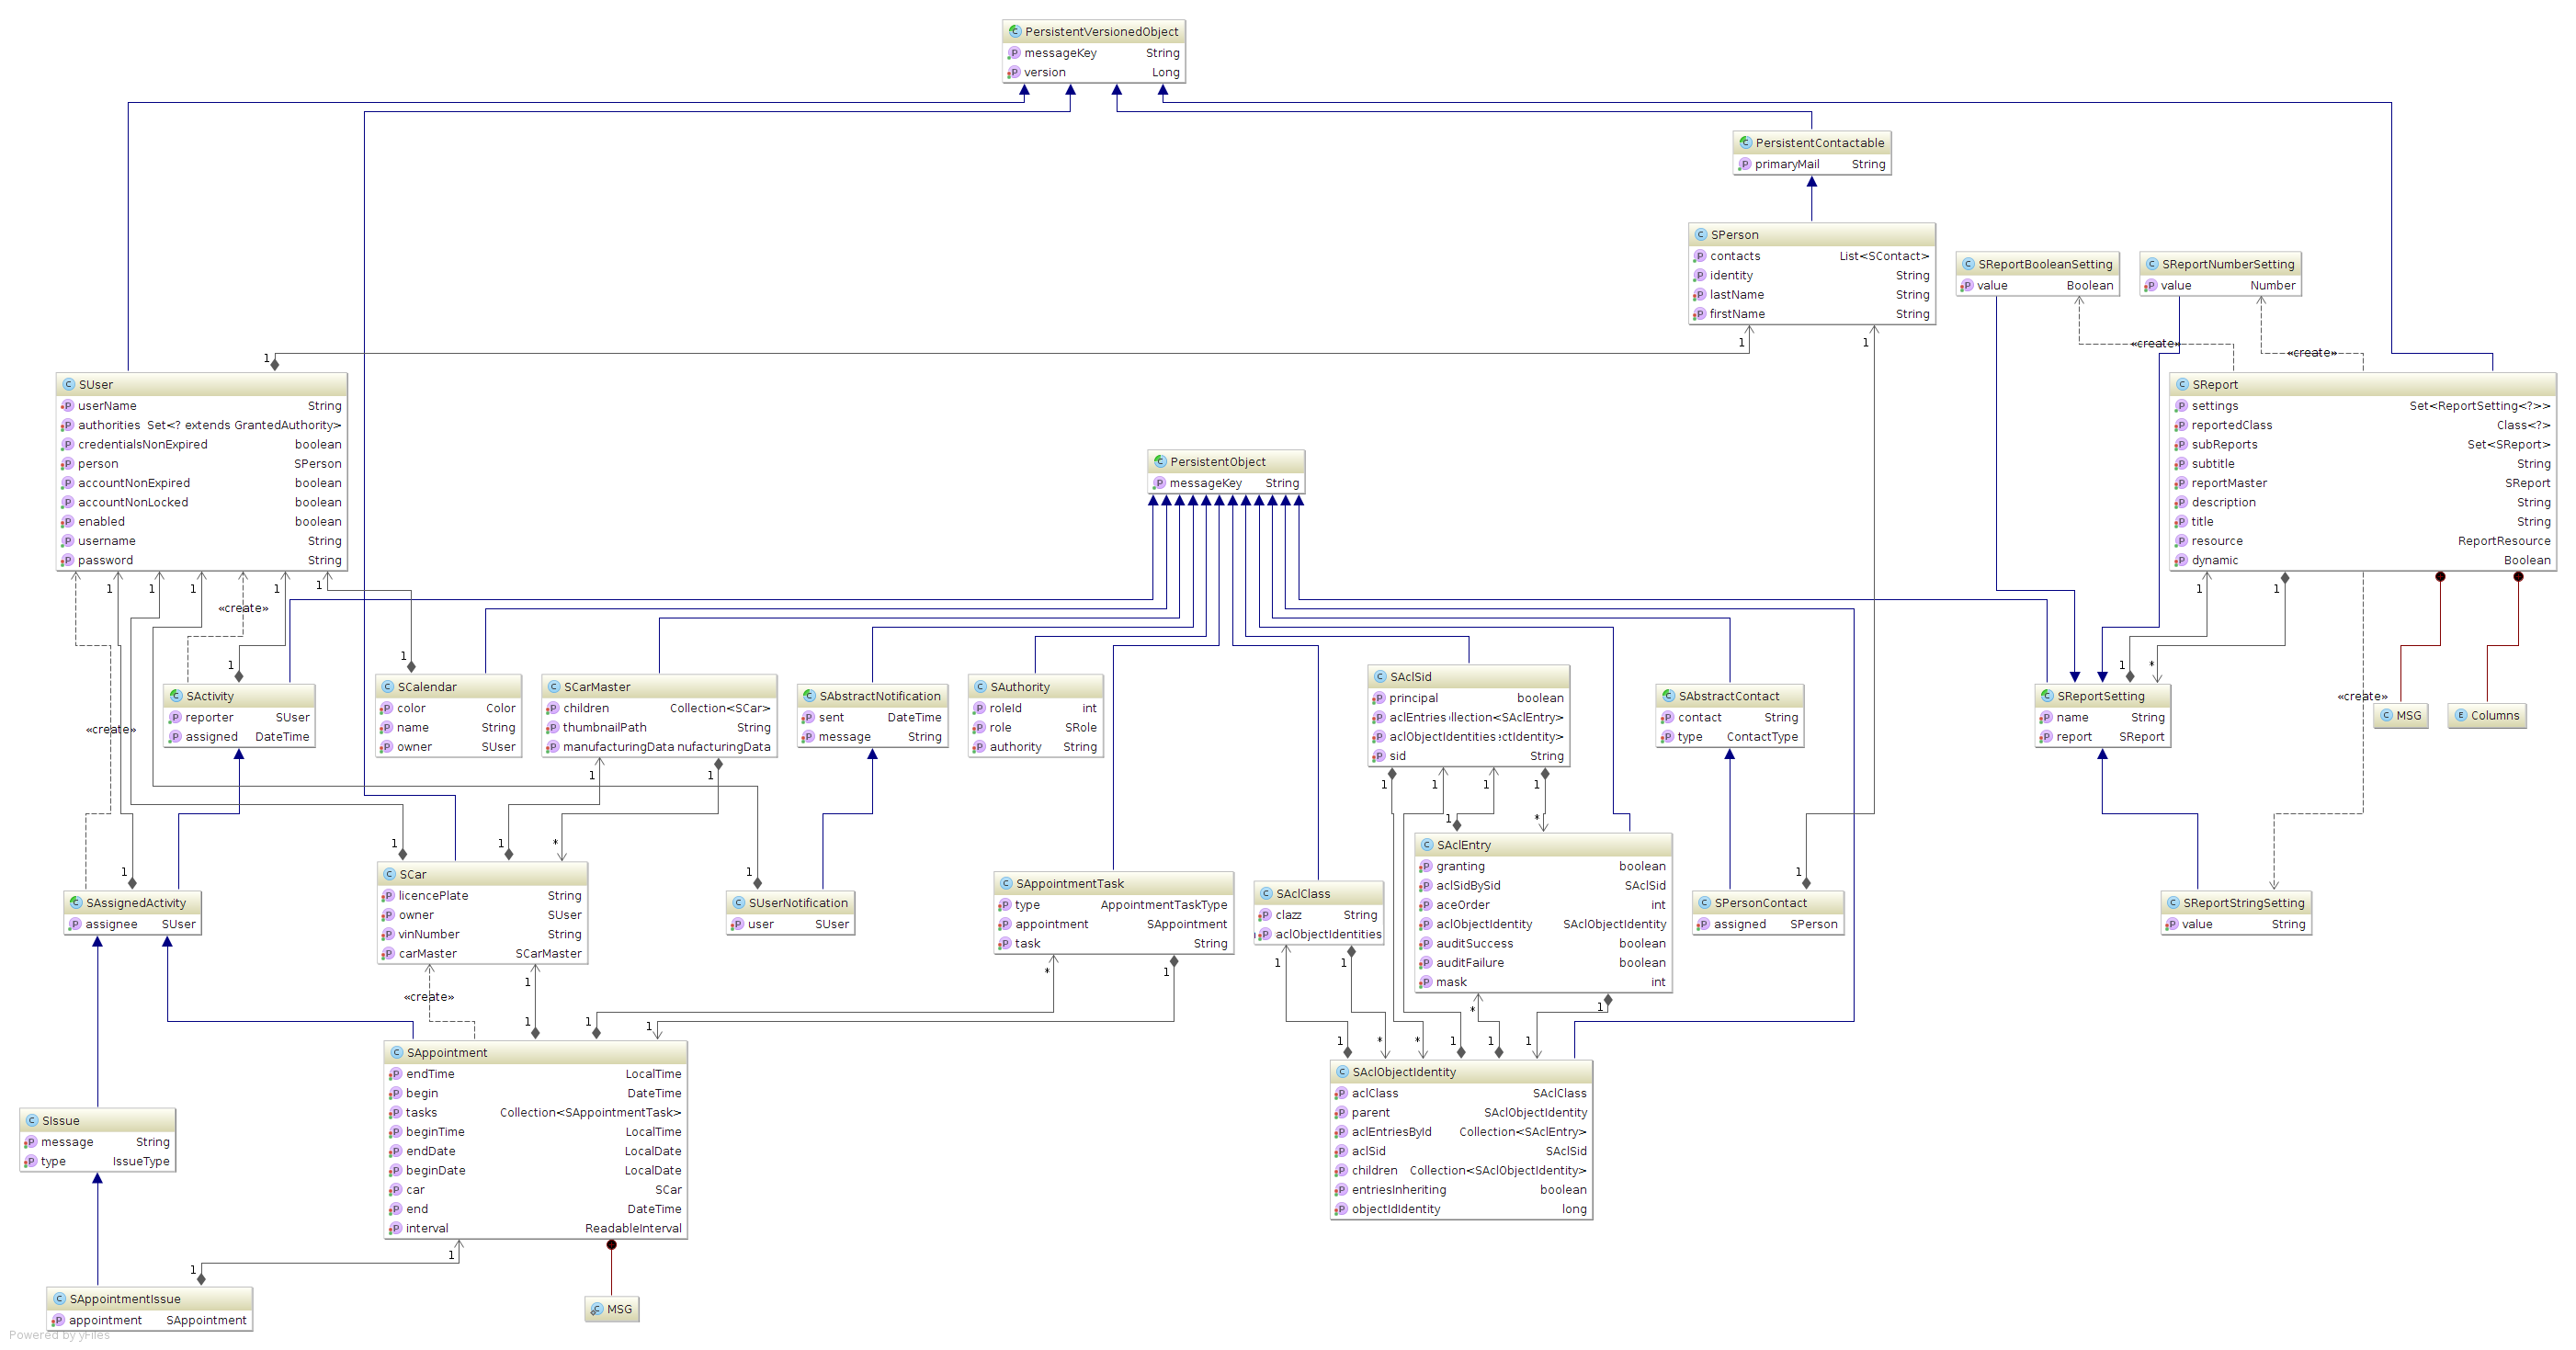
\includegraphics[angle=90,height=\textheight]{images/springatom_model_uml}
	\caption[Obiektowy model danych]{
		Obiektowy model danych odpowiadający\\który odpowiada schematowi bazy danych
	}
	\label{app:schema_org_agatom_springatom_model}
\end{figure}
\subsection{Schemat warstwy repozytoriów}
\begin{figure}[H]
	\centering
	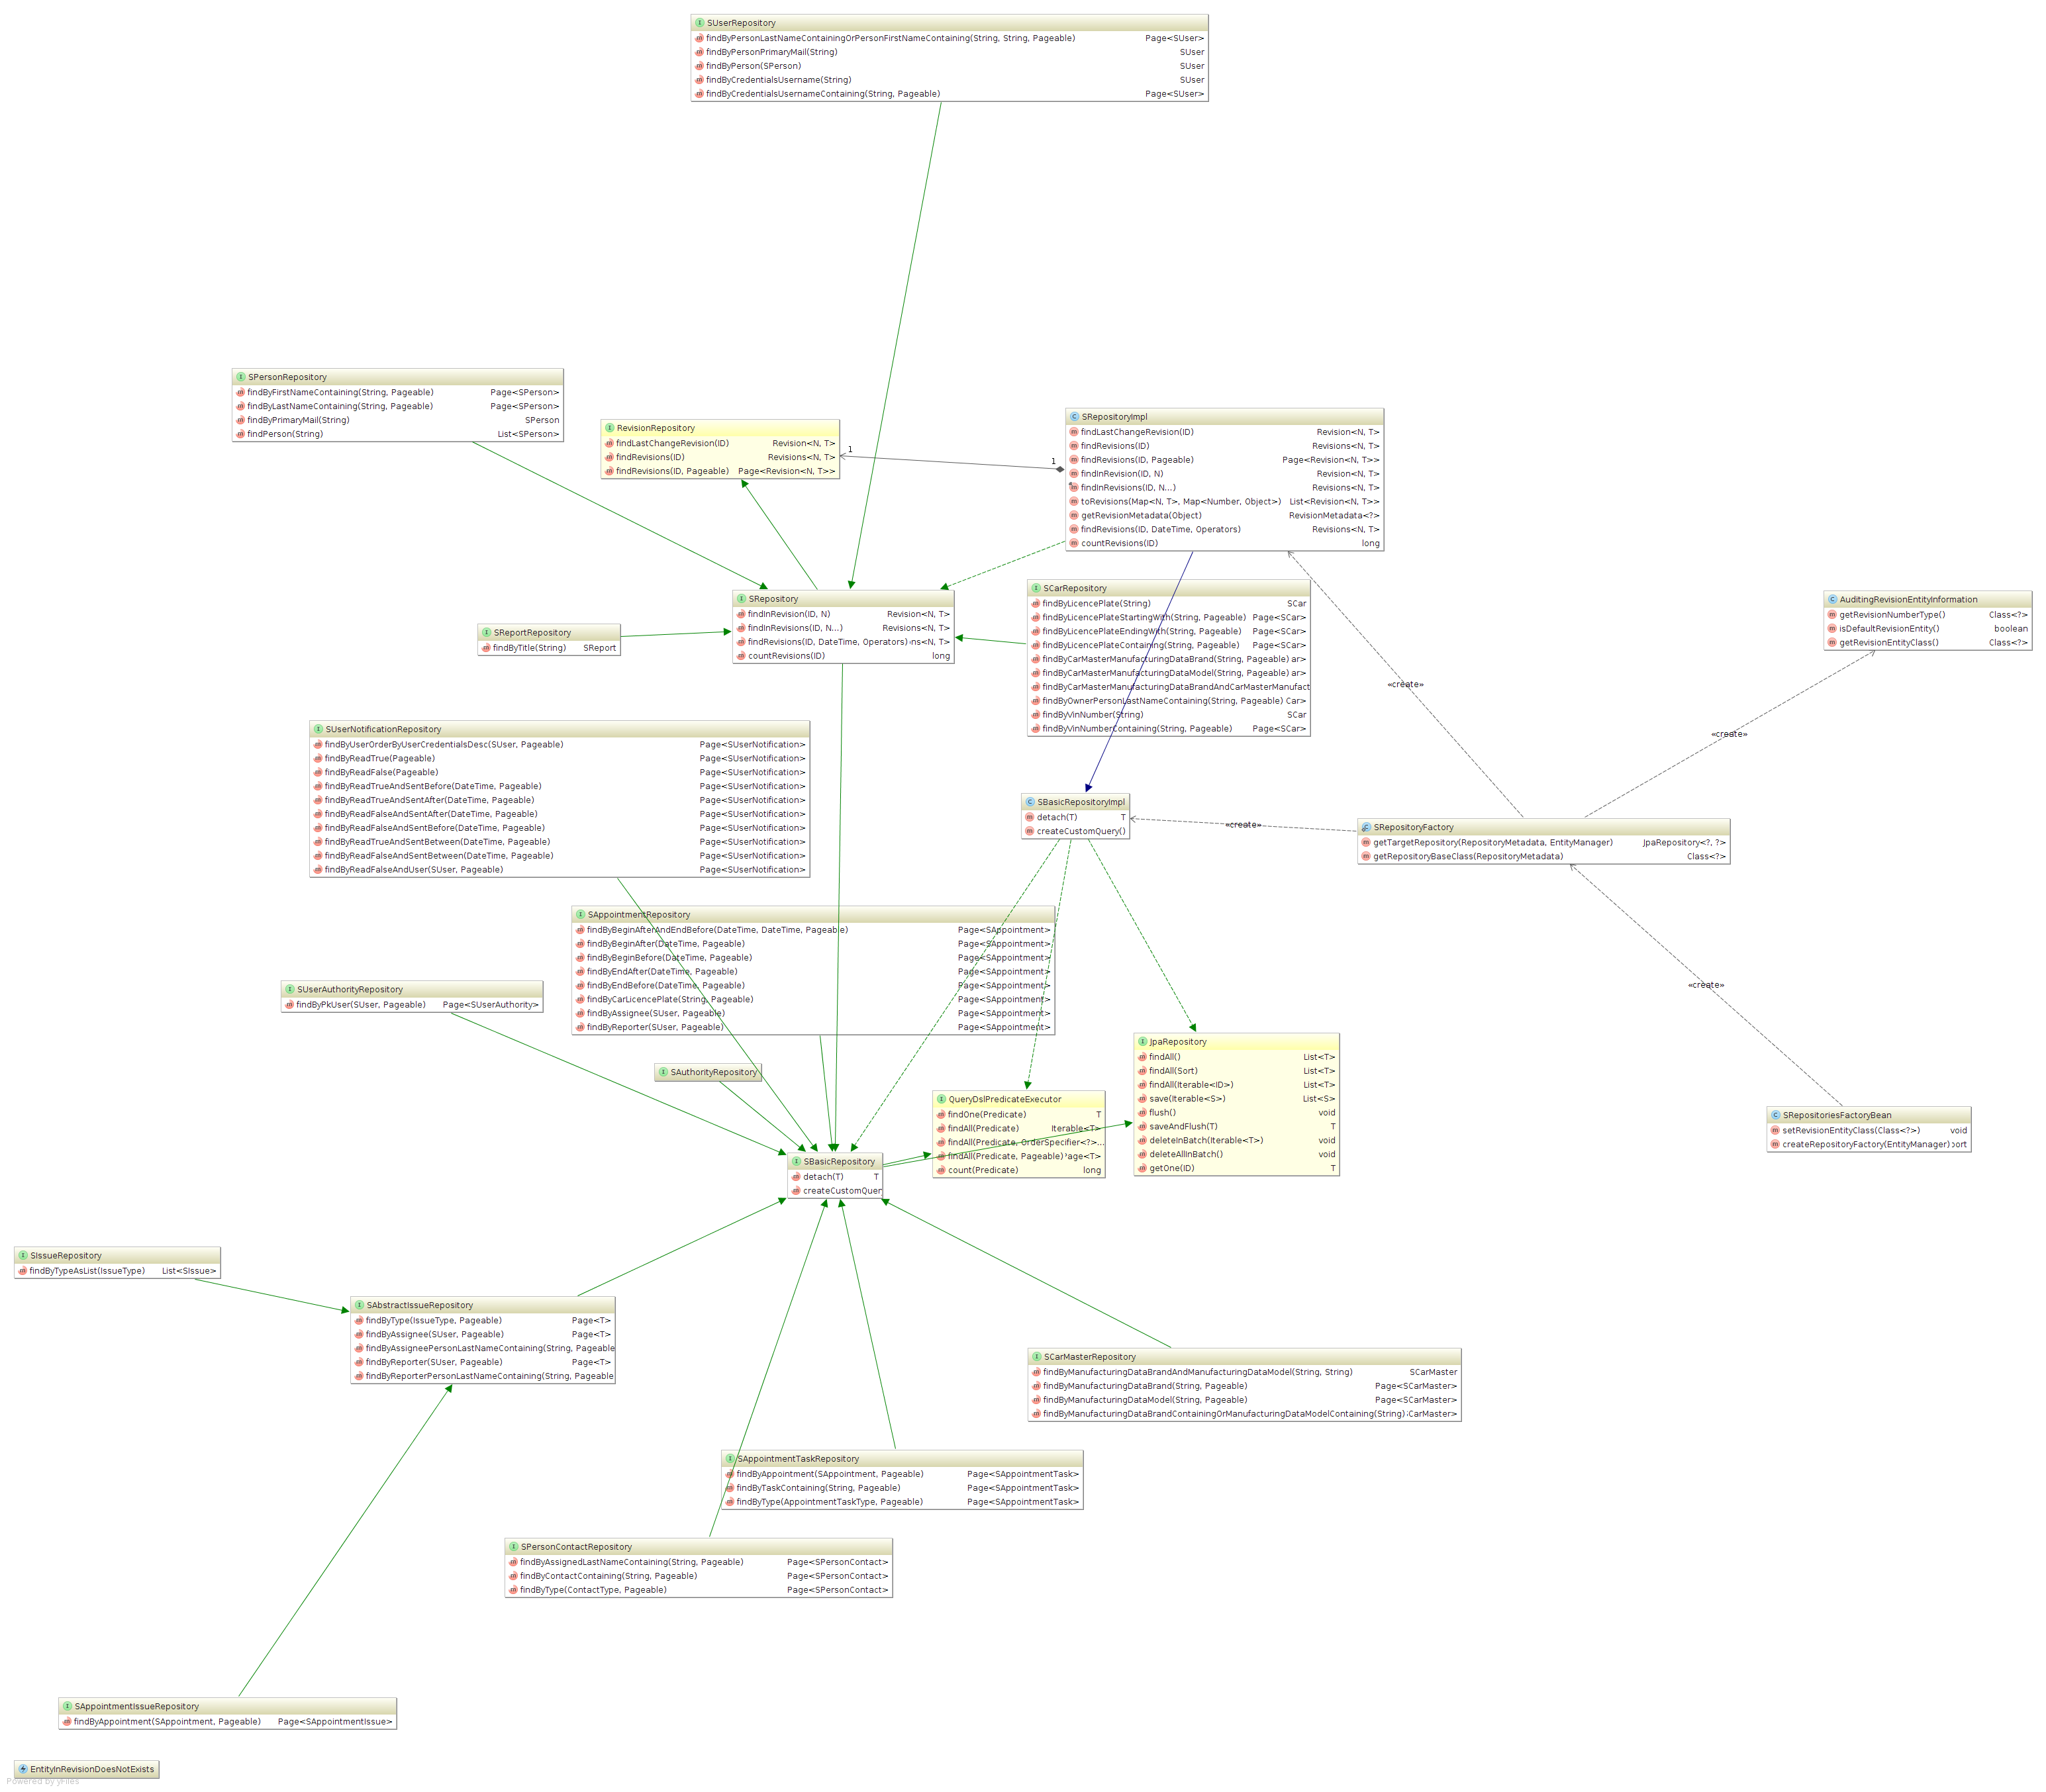
\includegraphics[width=\textwidth]{images/springatom_model_repository}
	\caption[Schemat repozytoriów aplikacji demonstracyjnej]{
		Schemat repozytoriów aplikacji demonstracyjnej
	}
	\label{app:schema_org_agatom_springatom_repository}
\end{figure}

\todo[inline]{Add the rest of UMLs}		
\section{Metryki kodu}												Kod aplikacji jest zbiorem funkcjonalności zaimplementowanych zarówno dla części serwerowej, jak i klienckiej. Z tego powodu liczba linii kodu
została podzielona na odpowiednie grupy, zgodne z językami użytymi do stworzenia aplikacji demonstracyjnej.
\subsection{Liczba linii kodu aplikacji}
\begin{center}
	\begin{longtable}{|l|l|l|l|l|}
		\caption[Liczba linii kodu według języka programowania]{
			Liczba linii kodu według języka programowania
		}
		\label{app:code_metric_loc}
		\tabularnewline	
		
		\hline
			\multicolumn{1}{|c|}{\textbf{Język}} 			&
			\multicolumn{1}{|c|}{\textbf{LOC}} 			&
			\multicolumn{1}{|c|}{\textbf{LOC (SC)}} 		&
			\multicolumn{1}{|c|}{\textbf{LOC (C)}} 		&
			\multicolumn{1}{|c|}{\textbf{LOC (EL)}} 		\tabularnewline
		\hline
		\endfirsthead
		
		\multicolumn{2}{c}
		{{\bfseries \tablename\ \thetable{} -- kontynuacja...}} \tabularnewline
		\hline
			\multicolumn{1}{|c|}{\textbf{Język}} 			&
			\multicolumn{1}{|c|}{\textbf{LOC}} 			&
			\multicolumn{1}{|c|}{\textbf{LOC (SC)}} 		&
			\multicolumn{1}{|c|}{\textbf{LOC (C)}} 		&
			\multicolumn{1}{|c|}{\textbf{LOC (EL)}} 		\tabularnewline
		\hline
		\endhead
			
		\hline
			\multicolumn{2}{|r|}{{Następna strona...}} \tabularnewline \hline
		\endfoot
		\hline
		\endlastfoot	
		
		\emph{Java}		& 29555	 	& 16628 	& 9136 		& 3791 	\hline
		\emph{JS} 		& 1044	 	& ? 		& ? 		& ? 	\hline
		\emph{JSP} 		& 2122	 	& ? 		& ? 		& ? 	\hline
		\emph{Razem} 	& 32721	 	& 16628 	& 9136 		& 3791  \hline
	\end{longtable}
	\begin{tabular}{l l}
			LOC 		& Całkowita liczba linii kodu 	\\
			LOC (SC)	& Liczba linii kodu źródłowego \\
			LOC (C)		& Liczba linii komentarzy		\\
			LOC (EL)	& Liczba linii pustych
	\end{tabular}	
\end{center}

\subsection{Java}
Tabela \ref{app:code_metric_loc} obrazuje złożoności projektu składającego się z 5 głównych modułów:
\begin{itemize}
	\item \textbf{AOP} - funkcjonalność opierająca się o \textit{Aspect Oriented Programming} zakresem obejmująca całą aplikację,
	\item \textbf{Core} - zbiór artefaktów (klas, klas abstrakcyjnych, interfejsów oraz typów wyliczeniowych) przeznaczonych do wykorzystania,
	\item \textbf{Server} - zadaniem klas tego modułu jest dostarczenie modelu danych, wsparcia jego walidacji oraz wersjonowania, definicji interfejsów repozytoriów, serwisów odpowiedzialnych za logikę biznesową,
	\item \textbf{Web} - artefakty tego modułu oferują definicje obiektów opisujących strony domenowe, tabele, przewodniki, raporty. Zawierają również klasy odpowiedzialne za
	dynamiczny i elastyczny model akcji. 
	\item \textbf{WebMVC}
\end{itemize}	

\subsubsection{Strukturalne metryki kodu}
\begin{center}
	\begin{longtable}{|l|l|l|l|l|l|}
		\caption[Liczba klas / Liczba linii kodu modułów]{
			Liczba klas / Liczba linii kodu modułów	
		}
		\label{app:modules_code_metrics}	
		\tabularnewline	
		
		\hline
			\multicolumn{1}{|c|}{\textbf{Moduł}} 			&
			\multicolumn{1}{|c|}{\textbf{LK}} 				&			
			\multicolumn{1}{|c|}{\textbf{LOC}}				&		
			\multicolumn{1}{|c|}{\textbf{CD}}				&	
			\multicolumn{1}{|c|}{\textbf{D}}				&
			\multicolumn{1}{|c|}{\textbf{TD}}				
			\tabularnewline
		\hline
		\endfirsthead
		
		\multicolumn{2}{c}
		{{\bfseries \tablename\ \thetable{} -- kontynuacja...}} \tabularnewline
		\hline
			\multicolumn{1}{|c|}{\textbf{Moduł}} 			&
			\multicolumn{1}{|c|}{\textbf{LK}} 				&			
			\multicolumn{1}{|c|}{\textbf{LOC}}				&		
			\multicolumn{1}{|c|}{\textbf{CD}}				&	
			\multicolumn{1}{|c|}{\textbf{D}}				&
			\multicolumn{1}{|c|}{\textbf{TD}}					
			\tabularnewline
		\hline
		\endhead
			
		\hline
			\multicolumn{2}{|r|}{{Następna strona...}} \tabularnewline \hline
		\endfoot
		\hline
		\endlastfoot	
		
		\emph{Aop}			&  3/3			& 	192/192			& 	0		& 	0		&	0		\hline
		\emph{Core}			&  13/1.86		& 	628/89.71		&	0		&	0.25	&	0.25	\hline
		\emph{Server}		&  187/3.07		& 	10806/183.15	&	0.82	&	3.32	&	23.48	\hline
		\emph{Web}			&  188/2.89		& 	10803/166.20	&	0.3		&	3.28	&	14.01	\hline
		\emph{WebMVC}		&  37/2.85		& 	2262/174		&	0		&	4.27	&	37.73	\hline
	\end{longtable}	
	\begin{tabular}{l l}
			LK 		& 	Liczba klas/Średnia liczba klas				\\
			LOC		& 	Liczba linii kodu/Średnia liczba linii kodu	\\
			D		& 	Średnia liczba cyklicznych zależności			\\
			CD		& 	Średnia liczba zależności						\\
			TD		& 	Średnia liczba zależności przechodnich			\\
	\end{tabular}	
\end{center}

\subsubsection{Metryka Chidamber-Kemerer}
Zadaniem metryki jest analiza następujących właściwości kodu \cite{chidamberKemerer}:
\begin{itemize}
	\item \textbf{WMC} - liczba metod zdefiniowanych w klasie,
	\item \textbf{DIT} - głębokość drzewa dziedziczenia,
	\item \textbf{SUB} - liczba bezpośrednich potomków w hierarchii dziedziczenia,
	\item \textbf{CBO} - stopień zależności od pozostałych artefaktów,
	\item \textbf{RFC} - ilość metod obiektu danej klasy, które mogę być wywołane w odpowiedzi na wywołania jednej metody tej klasy,
	\item \textbf{LCOM} - współczynnik kohezji, im wyższy, tym większa jest zależność między poszczególnymi artefaktami
\end{itemize}

\begin{center}
	\begin{longtable}{|l|l|l|l|l|l|l|}
		\caption[Metryka Chidamber - Kemerer]{
			Metryka Chidamber - Kemerer	
		}
		\label{app:chidamberKemerer}
		\tabularnewline	
		
		\hline
			\multicolumn{1}{|c|}{\textbf{Moduł}} 			&
			\multicolumn{1}{|c|}{\textbf{CBO}}				&		
			\multicolumn{1}{|c|}{\textbf{DIT}}				&	
			\multicolumn{1}{|c|}{\textbf{LCOM}}			&
			\multicolumn{1}{|c|}{\textbf{RFC}}				&	
			\multicolumn{1}{|c|}{\textbf{SUB}}				&
			\multicolumn{1}{|c|}{\textbf{WMC}} 			\tabularnewline
		\hline
		\endfirsthead
		
		\multicolumn{2}{c}
		{{\bfseries \tablename\ \thetable{} -- kontynuacja...}} \tabularnewline
		\hline
			\multicolumn{1}{|c|}{\textbf{Moduł}} 			&
			\multicolumn{1}{|c|}{\textbf{CBO}}				&		
			\multicolumn{1}{|c|}{\textbf{DIT}}				&	
			\multicolumn{1}{|c|}{\textbf{LCOM}}			&
			\multicolumn{1}{|c|}{\textbf{RFC}}				&	
			\multicolumn{1}{|c|}{\textbf{SUB}}				&
			\multicolumn{1}{|c|}{\textbf{WMC}} 			\tabularnewline
		\hline
		\endhead
			
		\hline
			\multicolumn{2}{|r|}{{Następna strona...}} \tabularnewline \hline
		\endfoot
		\hline
		\endlastfoot	
		
		\emph{Aop}			&  0		& 	1.00	& 	2.33	& 	12.00	&	0		&	6		\hline
		\emph{Core}			&  2.25		& 	1.50	&	1.00	&	34.60	&	0.62	&	5.12	\hline
		\emph{Server}		&  6.50		& 	2.35	&	1.64	&	282.30	&	0.77	&	7.16	\hline
		\emph{Web}			&  5.78		& 	2.03	&	1.74	&	194.33	&	0.64	&	7.47	\hline
		\emph{WebMVC}		&  5.00		& 	2.94	&	1.33	&	213.22	&	0.18	&	5.03	\hline
		\emph{Razem}		&  5.78		&	2.22	&	1.65	&	222.44	&	0.62	&	6.98	\hline
	\end{longtable}
\end{center}

Na uwagę zasługują w tym miejscu niskie wartości takich współczynników jak \textbf{DIT}, gdzie średnia wartość nie przekroczyła wartości 3, począwszy od korzenia wszystkich klas definiowanych w języku Java - \textbf{Object}. Przyjmuje się, że wartość graniczna dla większości aplikacji wynosi 5. Niemniej wartość średnia nie oddaje pojedynczych przypadków nadużyć. Większość takich sytuacji, występujących aplikacji demonstracyjnej, gdzie przekroczono graniczną wartość, odnosi się do klas rozszerzających standardowe możliwości szkieletu aplikacji, celem dostosowania ich do konkretnych przypadków użycia. Ponadto ważna jest głębokość drzewa dziedziczenia, przekraczająca przyjętą wartość w klasach opisujących biznesowy model danych. Fakt ten można pominąć z uwagi na to, że wspomniane artefakty służą wsparciu dla dziedziczenia wspólnych atrybutów dla konkretnych gałęzi klas oraz tym, że są to w klasy definiujące, prócz wspomnianych już pól, metody dostępowe, popularnie nazywane \textbf{gettery} oraz \textbf{settery}. W nielicznych przypadkach część funkcjonalności biznesowej została zamknięta w obiektach domenowych z uwagi na rozbieżność w sposobie przechowywania danych, a tym, jak są one udostępniane innym klasom. 

W tym miejscu warto wspomnieć o wartości jaką uzyskano dla wskaźnika \textbf{SUB}, który jest blisko związany z poprzednio omawianym \textbf{DIT}. Podczas gdy \textbf{DIT} opisuje głębokość drzewa dziedziczenia, co przekłada się na zwiększenie zarówno ilości atrybutów, jak i metod będących kandydatami do ponownego wykorzystania (nadpisania), \textbf{SUP} odnosi się do szerokości drzewa dziedziczenia, czyli ilości dzieci będących bezpośrednimi potomkami analizowanej klasy. Przyjęto, że niska wartość \textbf{DIT} jest zdecydowanie lepsza od \textbf{SUB}. Tak też jest w przypadku aplikacji demonstracyjnej, gdzie wartości tych dwóch współczynników charakteryzują się następującymi wartościami \textbf{DIT} równe 2.22, a \textbf{SUB} - 0.62. Widać wyraźnie, że zdecydowana większość klas definiuje swoją rolę poprzez mechanizm polimorfizmu.

Największym problem aplikacji okazała się wysoka wartość współczynnika \textbf{RFC}. Im jest ona wyższa, tym bardziej aplikacja narażona jest na błędy, a istniejąca złożoność utrudnia zrozumienie oraz testowanie aplikacji. 

\subsubsection{Metryka MOOD}
Metryki \textbf{MOOD} zostały zaprojektowane do mierzenia jakości aplikacji realizowanych z użyciem technik programowania obiektowego \cite{moodMetrics}. Analiza projektu nimi jest szczególnie użyteczna dla obszernych projektów. Duża ilość klas oraz istniejące plany rozwojowe sugerujące dalszy wzrost ilości linii kodu sprawiają, że stanowi ona cenna źródło wiedzy o strukturze programu i możliwości poprawienia rejonów szczególnie ważnych w kontekście właściwego wykorzystania paradygmatu programowania obiektowego.  
\begin{center}
	\begin{longtable}{|l|l|l|l|l|l|l|}
		\caption[Metryka MOOD]{Metryka MOOD}
		\tabularnewline	
		
		\hline
			\multicolumn{1}{|c|}{\textbf{AHF}}				&		
			\multicolumn{1}{|c|}{\textbf{AIF}}				&	
			\multicolumn{1}{|c|}{\textbf{CF}}				&
			\multicolumn{1}{|c|}{\textbf{MHF}}				&	
			\multicolumn{1}{|c|}{\textbf{MIF}}				&
			\multicolumn{1}{|c|}{\textbf{PF}} 				\tabularnewline
		\hline
		\endfirsthead
		
		\multicolumn{2}{c}
		{{\bfseries \tablename\ \thetable{} -- kontynuacja...}} \tabularnewline
		\hline
			\multicolumn{1}{|c|}{\textbf{AHF}}				&		
			\multicolumn{1}{|c|}{\textbf{AIF}}				&	
			\multicolumn{1}{|c|}{\textbf{CF}}				&
			\multicolumn{1}{|c|}{\textbf{MHF}}				&	
			\multicolumn{1}{|c|}{\textbf{MIF}}				&
			\multicolumn{1}{|c|}{\textbf{PF}} 				\tabularnewline
		\hline
		\endhead
			
		\hline
			\multicolumn{2}{|r|}{{Następna strona...}} \tabularnewline \hline
		\endfoot
		\hline
		\endlastfoot	
		
		100.0\%{} 	& 
		0.00\%{} 	& 
		0.00\%{}	& 
		53.85\%{}	& 
		0.00\%{} 	& 
		100.0\%{} 	\tabularnewline
	\end{longtable}
	\label{app:moodMetrics}
	\begin{tabular}{l l}
			AHF 	& 	Współczynnik enkapsulkacji pól klas			\\
			AIF		& 	Współczynnik dziedziczenia atrybutów			\\
			CF		& 	Współczynnik powiązań							\\
			MHF		& 	Współczynnik enkapsulkacji metod				\\
			MIF		& 	Współczynnik dziedziczenia metod				\\
			PF		& 	Współczynnik polimorfizmu						\\
	\end{tabular}	
\end{center} 

Na istotną uwagę zasługują dwa wskaźniki \textbf{PF=100\%{}} oraz \linebreak \textbf{MHF=53.85\%{}}. Pierwszy z wyników odnosi się do polimorfizmu. Wynik z pewnością wskazuje na dobry projekt systemu wykazującego duży poziom abstrakcyjność, co usprawnia późniejsze modyfikacje na poziomie zmiany sposobów realizacji konkretnych bloków funkcjonalnych. Stałym artefaktem podczas takiej zmiany jest interfejs, definiujący kontrakt konkretnej gałęzi klas, podczas gdy zmiana zachodzi na poziomie poszczególnych jego implementacji.

 Drugi ze wskaźników odnosi się do współczynnika enkapsulacji metod. Obliczany jest z następującego wzoru: \[ MHF = 1 - \frac{\sum{MV}}{(C-1)} \] \textbf{MV} - liczba klas, gdzie dana metoda jest widoczna oraz \textbf{C} - ilość klas. Nie ma jednoznacznie przyjętej poprawnej wartości tej metryki, niemniej uznaje się, że im wyższa wartość tym jakość kodu jest większa, a potencjalne błędy skupione i łatwe do zlokalizowania. Z drugiej strony wysoka wartość oznacza wysoką specjalizację klas przy jednocześnie niskim poziomie funkcjonalności, która rozsiana jest między poszczególnymi elementami systemu. 